%Document vide aux normes de l'École nationale des Chartes
%Dernières modifications Maxime Rolland (09/2024)

%%%%%%%%%%%%%%%%%%%%%% PRÉAMBULE


%%%%%%%%%%%%%% partie obligatoire du préambule
\documentclass[a4paper,12pt,twoside]{book}
\usepackage{fontspec}
\usepackage{xunicode}
\usepackage[english,french]{babel}%on peut préciser d'autres langues.


%%%%%%%%%%%%%%%%%%%%%%%%%%%%%%%%% PACKAGES UTILISÉS

\usepackage{csquotes} % les guillemets français
\usepackage{lettrine} %faire une lettrine (pas obligatoire)

\usepackage[backend=biber, sorting=nyt, style=enc, minbibnames=10, maxbibnames=10, style=verbose]{biblatex}
\addbibresource{Bibliographie/collab.bib}
\addbibresource{Bibliographie/DB - BD.bib}
\addbibresource{Bibliographie/Demo.bib}
\addbibresource{Bibliographie/DL.bib}
\addbibresource{Bibliographie/PPP.bib}

\nocite{*}
\defbibnote{intro}{Cette bibliographie liste les ressources utilisées, classées par thème et citées par ordre alphabétique.}

%%%Faire un ou plusieurs index

%\usepackage{imakeidx} %pour faire un ou plusieurs index
%\makeindex %commande pour générer l'index
%-> Choix de ne pas ajouter d'index, qui ne nous paraissait pas nécessaire. 


%RAJOUTEZ ICI VOS PACKAGES
\usepackage{float}% Forcer la position de la figure
\usepackage{array} % Pour des options de mise en forme avancées des tableaux
\usepackage{booktabs}% Améliorer l'apparence des tableaux
\usepackage{enumitem} % Pour avoir des bullets points
\usepackage{fancyvrb} % Pour le style de texte en mode code
\usepackage{pdfpages} % Pour importer des PDF
\usepackage{graphicx} % Pour ajouter des images d'illustrations
\usepackage{caption} % Pour la légende des figures
\usepackage{fancybox} % Pour ajouter des cadres décoratifs
\usepackage{setspace} % Pour ajuster l'espacement si nécessaire





%%%%%%%%%%%%%%%%%%%%%%%%%%%%%%%%% CONFIGURATION DE MISE EN PAGE

%%%%%% Les compteurs (sections, subsections, etc)
\renewcommand{\thesection}{\Roman{section}.}%On ne fait apparaître que le numéro de la section
\renewcommand{\thesubsection}{\arabic{subsection}.}%subsection en chiffres arabes
\renewcommand{\thesubsubsection}{\alph{subsubsection}.}%subsubsection en lettres minuscules
%Si l'on veut faire apparaître les subsubsection dans le table des matières (à commenter sinon)
\setcounter{tocdepth}{3}
\setcounter{secnumdepth}{3}  % La subsubsection (profondeur=3 dans la table des matières) apparait numérotée dans la TdM

%%%%%  Configurer le document selon les normes de l'école

\usepackage[margin=2.5cm]{geometry} %marges
\usepackage{setspace} % espacement qui permet ensuite de définir un interligne
\onehalfspacing % interligne de 1.5
\setlength\parindent{1cm} % indentation des paragraphes à 1 cm

%%%%% Mise en forme des headers (haut de page)

\usepackage{fancyhdr} %package utilisé pour modifier les headers
\pagestyle{fancy} %utiliser ses propres choix de mise en page et non ceux par défaut du package

\setlength\headheight{16pt}%la hauteur des headers
%\renewcommand{\sectionmark}[1]{\markright{\small\textit{\thesection~\  #1}}}%Faire apparaître dans les headers les sections en  petit et en italiques
\renewcommand{\sectionmark}[1]{}%Commenter la lign précédetne et mettre celle-ci pour ne pas avoir le titre des sections dans le header
\renewcommand{\chaptermark}[1]{\markboth{\small\chaptername~\thechapter~--\ \textit{#1}}{}}%idem pour les chapitres
%\renewcommand{\chaptermark}[1]{}%Commenter la ligne précédente et mettre celle-ci pour ne pas avoir le titre des chapitres  dans le header


%%%%%%% Package hyperref

%avec overleaf, utiliser :
\usepackage[xetex]{hyperref}

%%%%%%%%%%%%%%%%%%%% Package glossaries

%Exception: il faut le charger APRÈS hyperref
\usepackage[toc=true, acronym]{glossaries}%Options qui permettent d'ajouter le glossaire à la table des mattières, et de mettre des acronymes 
\makeglossaries

\loadglsentries{Glossaire.tex}

%%%%%%%%%%%%%%%%%% DÉFINITION DES COMMANDES ET ENVIRONNMENTS
%%%%Pour faire apparaitre le nom des outils dans une police particulière%%%%%%
\newcommand{\Arkindex}{\texttt{Arkindex}}
\newcommand{\Spider}{\texttt{Spider}}
\newcommand{\DAN}{\texttt{DAN}}
\newcommand{\YOLO}{\texttt{YOLO}}

 %%%%%%%%%%%%%% INFORMATIONS POUR LA PAGE DE TITRE
\author{Maxime Rolland - M2 TNAH}
\title{Titre du mémoire}

%%%%%%%%%%%%%%%%%%%%%% DOCUMENT
\begin{document}
	\begin{titlepage}
		\begin{center}
			
			\bigskip
			
			\begin{large}				
				ÉCOLE NATIONALE DES CHARTES\\
				UNIVERSITÉ PARIS, SCIENCES \& LETTRES
			\end{large}
			\begin{center}\rule{2cm}{0.02cm}\end{center}
			
			\bigskip
			\bigskip
			\bigskip
			\begin{Large}
				\textbf{Maxime Rolland}\\
			\end{Large}
		%selon le cas
			\begin{normalsize} \textit{licenciée en histoire}\\
				\textit{diplômée de master}
			\end{normalsize}
			
			\bigskip
			\bigskip
			\bigskip
			
			\begin{Huge}
				\textbf\textbf{CENT ANS DE RECENSEMENT FRANÇAIS EN UNE BASE DE DONNEES, L’EXEMPLE SOCFACE}\\
			\end{Huge}
			\bigskip
			\bigskip
			\begin{LARGE}
				\textbf{Interdisciplinarité et recherche partenariale au service du traitement de données à grande échelle}\\
			\end{LARGE}
			
			\bigskip
			\bigskip
			\bigskip
			\begin{large}
			\end{large}
			\vfill
			
			\begin{large}
				Mémoire 
				pour le diplôme de master \\
				\enquote{Technologies numériques appliquées à l'histoire} \\
				\bigskip
				2024
			\end{large}
			
		\end{center}
	\end{titlepage}

	\thispagestyle{empty}	
	\cleardoublepage
	
\frontmatter



	\chapter{Résumé}
\medskip
	Ce mémoire explore le projet SocFace, une initiative collaborative entre l'INED, Teklia, le SIAF et PSE, visant à numériser et analyser les listes de recensement français de 1836 à 1936. Le projet se distingue par son utilisation de technologies de pointe, notamment le deep learning, pour traiter un volume massif de données historiques. L'étude met l'accent sur l'interdisciplinarité et la collaboration entre les secteurs public et privé, examinant comment ces dynamiques influencent la gouvernance des données et l'intégrité des résultats. Le mémoire analyse également les défis liés à l'intégration et à la valorisation des données dans un environnement de recherche interdisciplinaire.\\

    This thesis explores the SocFace project, a collaborative initiative between INED, Teklia, SIAF, and PSE, aimed at digitizing and analyzing French census lists from 1836 to 1936. The project stands out for its use of cutting-edge technologies, including deep learning, to process a massive volume of historical data. The study focuses on interdisciplinarity and the collaboration between public and private sectors, examining how these dynamics influence data governance and the integrity of results. The thesis also addresses the challenges of data integration and valorization in an interdisciplinary research environment.\\
	
	\textbf{Mots-clés: Archives ; Base de données ; Big Data ; Démographie ; Deep Learning ; INED ; Interdisciplinarité ; LLM ; Metabase ; PPP ; Recensement ; Teklia}.
	
	\textbf{Informations bibliographiques:} Maxime Rolland, \textit{ Cent Ans de recensement français en une base de données, l’exemple SocFace. L’interdisciplinarité et le partenariat Public/Privé au service du traitement de données à grande échelle }, mémoire de master \enquote{Technologies numériques appliquées à l'histoire}, dir. [Ségolène Albouy, Lionel Kesztenbaum], École nationale des chartes, 2024.
	
		\newpage{\pagestyle{empty}\cleardoublepage}
	
	\newpage{\pagestyle{empty}\cleardoublepage}
	
	\chapter{Remerciements}
	
\lettrine{M}es remerciements vont tout d'abord à Lionel Kesztenbaum, qui m'a accueillie au sein de l'INED et de SocFace et qui m'a transmis sa passion pour le projet et pour la recherche. Je le remercie également pour le temps passer à la relecture de ce mémoire et m'avoir gardé des écueils dans lesquels j'ai été tenté de tomber. Je remercie également Christopher Kermorvan, dont la pédagogie et la disponibilité m'ont permis de comprendre facilement une technologie complexe, ainsi que tous les membres de l'équipe. Ce mémoire est l'aboutissement d'une année intense, qui a été rendue plus douce par la meilleure classe de master possible. J'y ai trouvé l'entraide nécessaire, le soutien et la joie qui m'ont aidé à surmonter les heures d'intense réflexion sur des sujets que je ne suis toujours pas sûre de maîtriser. Mes remerciements vont également à Madame Bermès et à toute l'équipe pédagogique du master, particulièrement Ségolène Albouy, dont les conseils m'ont habilement guidé pour l'écriture de ce mémoire. Sa rigueur et ses réponses à mes questionnements ont été d'une précieuse aide. \\
Je remercie ma famille et mes proches qui ont subi mes angoisses durant cette année et surtout pendant l'écriture de ce mémoire. 
Enfin, je remercie tout particulièrement Matthieu, qui m'a supporté - dans tous les sens du terme - durant cette longue année. Que sa patience soit érigée en modèle. Également Bacon et Billy, dont la présence ronronnante ont rythmé mon écriture cet été. \\

Ce travail est l'aboutissement d'une longue reconversion, qui n'aurait pas été possible sans mon Grand-Père. Ce mémoire lui est dédié. 

	\newpage{\pagestyle{empty}\cleardoublepage}

\begingroup
    \let\cleardoublepage\clearpage
% Appel des bibliographies une par une avec un titre différent pour chacune
    \printbibliography[keyword={Collab}, title={Collaboration et Interdisciplinarité}]
    \printbibliography[keyword={DB - BD}, title={Base de Données et Big Data}]
    \printbibliography[keyword={Demo}, title={Démographie}]
    \printbibliography[keyword={PPP}, title={Recherche Partenariale}]
    \printbibliography[keyword={DL}, title={Deep Learning}]
\endgroup

\newpage{\pagestyle{empty}\cleardoublepage}%Evite le doublement des titres dans un en-tête
	
\chapter{Introduction}	
Marcel Proust écrivait dans \textit{Du côté de chez Swann} que \textit{"Le véritable voyage de découverte ne consiste pas à chercher de nouveaux paysages, mais à avoir de nouveaux yeux".} En suivant cette recommandation, le projet SocFace, porté par l'\gls{INED}, Teklia, le \gls{SIAF} et \gls{PSE}, nous offre la possibilité de redécouvrir un vaste continent d'informations. Ce projet ambitieux vise à rendre accessibles l'ensemble des données des recensements français de 1836 à 1936, représentant des millions d'enregistrements. Grâce à une base de données, ces précieuses informations pourront être explorées et analysées en profondeur, permettant une compréhension globale inédite de cette période.\\

L’objectif de ce mémoire n’est pas de disséquer la technologie mise en oeuvre dans le projet SocFace ou de replacer celui-ci dans l’évolution de l'\gls{HTR}. Ce qui nous a paru intéressant d’étudier dans ce projet, c’est l’aspect organisationnel : la façon dont différents acteurs et outils dialoguent ensemble. SocFace est un projet multidisciplinaire, à double titre. Plusieurs disciplines dites « académiques » dialoguent, de façon assez courante dans un projet de recherche. Ce n’est bien évidemment pas rare pour un projet de recherche. Mais ici, la spécificité est que ce dialogue est ouvert à un autre acteur, spécialisé en ingénierie informatique, un domaine moins familier des projets de recherche. Cette multi-disciplinarité se double d’une collaboration entre institutions publiques et entreprises privées, un autre aspect singulier de ce projet. Trois axes vont donc conduire notre réflexion : l’interdisciplinarité, la collaboration et la recherche partenariale. Il est intéressant de comprendre comment la collaboration, entre des entités différentes, se déroule au service d’un projet commun. Pour autant, il faut bien différencier interdisciplinarité, qui concerne le domaine de recherche d’une institution, d’un chercheur, et collaboration, terme davantage utilisé dans le cadre de la gestion de projet. Les relations entre Teklia, l’entreprise privée porteuse du projet et l’INED sont une collaboration interdisciplinaire, et également un partenariat entre public et privé. Les relations entre l’INED et le SIAF sont entendues comme une collaboration, mais ce n’est évidemment pas un partenariat public/privé. On comprend donc que ces différentes dimensions se recroisent et se recoupent mais sont bien distinctes. \\
L’autre aspect singulier de SocFace, c’est l’ampleur des données qu’il doit traiter. On parle à la fois des sources, issues de l’ensemble des archives françaises, mais également des données produites à l’issue du processus \gls{HTR}\footnote{Voir Glossaire}. On parle ici d’\gls{HTR} car les livres de recensement sont remplit à la main, même jusqu’en 1936. Cette caractéristique - et le fait qu’il s'agisse de millions d’entités spécifiques -  nécessite l’utilisation du \gls{ML}\footnote{Voir Glossaire} et de l'apprentissage supervisé de l'intelligence artificielle. L’application de cette technologie pour extraire les données, et le fait que plusieurs équipes travaillent sur le processus oblige à s’interroger sur leur intégrité. On ne peut d’ailleurs dissocier cette donnée des différents outils développés par les équipes du projet pour le processus \gls{HTR}. Comprendre le fonctionnement de ces outils permet de comprendre la nature de la donnée à l’issue de la mise en production. Ce qui nous intéresse ici, c’est étudier ce fonctionnement dans le cadre d’une collaboration à différents acteurs et comment cela impacte la donnée. \\
La donnée est véritablement au cœur du projet, conférant à SocFace une portée exceptionnelle, à la fois dans ces objectifs, et dans les technologies développées pour les atteindre. Ainsi, l’un des ultime objectifs – qui demande des développements d’outils de pointe – est l’appariement. Cette technique permet de relier les données, notamment celles concernant les individus, afin de retracer leurs trajectoires à travers l'espace et le temps. Le nom du projet – traduit en anglais - illustre d'ailleurs cette ambition : \textit{The local \textbf{\underline{FACE}} of \textbf{\underline{SOC}}ial change: one century of French social structure seen from the ground, 1836-1936}. Au-delà de cet usage spécifique, la base de données pourrait également devenir une ressource précieuse pour d'autres chercheurs, leur offrant la possibilité de mener des analyses sociales, économiques et géographiques sur la France de cette époque. Si notre analyse se concentre davantage sur les moyens humains que sur les technologies, les outils développés pour le projet marquent une avancée dans le domaine de l’\gls{HTR}. Il est donc intéressant de voir dans quels autres domaines ou projets du patrimoine ces outils pourront être utilisés, car ils sont une ressource précieuse pour les humanités numériques. Ces avancées, permises par l’interdisciplinarité et le dialogue entre deux types de professionnels doivent être replacées cela dans l’écosystème plus vaste du monde de la recherche. \\

Ainsi, SocFace est un vaste projet aux multiples acteurs. Ces acteurs appartiennent à différentes sphères de la recherche, et mettent leur collaboration au service de la production d’une somme de données considérable. Tous ces éléments nous invitent à nous interroger sur leur articulation : 
en quoi le projet SocFace s'appuie-t-il sur l'interdisciplinarité et la collaboration entre institutions publiques et entreprise privée, pour réaliser l'extraction de données et créer une base de données à très grande échelle ?  Cette problématique vise à interroger l’intérêt de l’interdisciplinarité pour les projets mettant en jeu un volume de données. Est-ce nécessaire ou au contraire, une complication dans le pilotage du projet ? et quel est l’impact sur la gouvernance des données, notamment leur intégrité ?\\

Pour répondre à ces questions nous poserons tout d’abord les bases du projet, afin de mieux comprendre son fonctionnement. Ici, on parle de l’articulation des acteurs entre eux, et leur rapport les uns aux autres. Puis nous entrerons davantage au cœur du projet, à savoir l’exploration de la donnée : sa nature, sa production, son chemin. Une fois ces éléments expliqués et analysés, il sera temps d’en tirer les conclusions, et notamment comment se positionne le projet au sein de la recherche actuelle : d’une part concernant les acteurs, et le dialogue interdisciplinaire qui les lie, et d’autre part concernant le résultat du projet : les données produites et les outils développés pour le faire. 
\newpage{\pagestyle{empty}\cleardoublepage}

%%%%%%%%%%%%%%%%%Le corps du mémoire
	\mainmatter

	\part{Comment le projet SocFace intègre-t-il l'interdisciplinarité?}

 SocFace est un projet interdisciplinaire. Ce n’est pas exceptionnel dans le domaine de la recherche actuelle, mais il faut néanmoins comprendre comment cette interdisciplinarité s’articule autour d’un objectif commun. Nous devons également aborder la notion de collaboration, et étudier comment plusieurs équipes, aux compétences et fonctionnement différents, travaillent ensemble. Cela permet de mettre en lumière la singularité de chacune des équipes, et notamment ce qui les oppose le plus franchement : l’appartenance au secteur privé pour l’une et au secteur public pour les autres. 
\vspace*{\fill}
\begin{center}
  % Ajouter un joli cadre autour de l'image
  \setlength{\fboxsep}{5pt}  % Espace entre l'image et le cadre
  \setlength{\fboxrule}{1pt} % Épaisseur du cadre
  \fbox{
    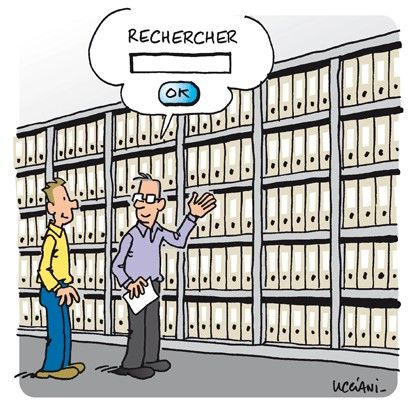
\includegraphics[width=0.8\textwidth]{Figures/Partie 1/Illus.Partie 1.jpeg}}\\
    \vspace{0.5em} % Espace entre l'image et la légende
    {\scriptsize \textit{Crédit : Ucciani dessins.}}
\end{center} 
\chapter{Quid du projet SocFace?}
L’objectif de SocFace est très simple : numérisation des listes de recensements français de 1836 à 1936 et extraction des informations pour créer une base de données. Ce qui est moins évident, c’est d’une part la mise en œuvre et d’autre part, la gestion des résultats escomptés. Ce sont de fait les chiffres qui impressionnent le plus et qui font toute la singularité de SocFace. On se demandera d’ailleurs si on peut parler de Big Data pour les données du projet. 



    \section{Objectifs du projet}

Les listes des \gls{LNR}\footnote{Voir Glossaire} sont conservées en grande majorité dans les Archives Départementales et les Archives Municipales des grandes villes. L’un des objectifs du projet est donc de favoriser la collaboration entre les services d’archives et les acteurs du projet. La très grande majorité de ces archives avaient déjà numérisé les listes de recensement.\\
Le principe de dénombrement via le recensement commence en 1836. Il est à noter que quelques expériences avaient été tentées auparavant : des dénombrements fiscaux, des enquêtes par les intendants, sous Louis XIV et Louis XV. Mais ces listes sont des initiatives locales et n'ont pas le caractère imposé, sériel et national des listes de recensement qui commencent en 1836. Ces listes se font par commune et dénombrent individuellement la population. Elles sont classées par rues, puis chaque habitant est dénombré par famille : le chef de famille en tête, puis son épouse, ses enfants, et les autres membres du ménages, qu’ils soient membres de la famille
ou non (les personnes employées par le ménage, en particulier les domestiques, ou simplement logés par lui). Différentes informations sont fournies sur chaque individu, variable au cours du temps. Mais on retrouve de façon à peu près constante : le nom, prénom, âge (ou année de naissance), position dans la famille, profession et nationalité (depuis 1851).\\
    
    \begin{figure}[H]
        \centering
        \includegraphics[width=0.8\linewidth]{Figures/Partie 1/Fig.1.1 - LNR Eygalières.png}
        \caption[Extrait du recensement des Bouches du Rhône - de 1861 pour le village d'Eygalières]{Extrait du recensement des Bouches du Rhône de 1861 pour le village d'Eygalières}
        \label{fig:Fig1.1}
    \end{figure}

L’objectif principal est de produire une base de données qui reprend toutes ces informations. Les images sont classées par service fournisseur d'archives, en général au niveau départemental, puis par année et enfin par commune. La base de données permet donc de naviguer dans toutes ces informations et retrouver le nom d’un habitant en particulier, ou à l’inverse le nom de la commune et même de la rue dans laquelle habitait une personne. Ce type de recherche existe déjà, développé par la communauté des généalogistes. Les bases de données de ces communautés sont généralement basées sur des indexations d’état civil fait par des passionnés, "à la main". On y trouve des associations départementales, comme les bases RECIF pour le Finistère ou bien des logiciels à visée nationale comme Généanet\footnote{\href{https://www.geneanet.org/}{https://www.geneanet.org/}} ou MyHeritage\footnote{\href{https://www.myheritage.fr/}{https://www.myheritage.fr/}} (payants) ou ELIE\footnote{\href{https://www.mcs-gen.com/}{https://www.mcs-gen.com/}} (gratuit).\\

En France, d'autres projets ont adopté une démarche similaire.  Le CNRS, en partenariat avec le laboratoire informatique \gls{LITIS} porte le projet POPP, dont le périmètre est recentré sur Paris durant l’entre-deux guerres (1926-1946). Ce projet s’est doublé du projet EXO-POPP, qui concerne les actes de mariages de Paris et sa banlieue sur la même période. Un immense projet a également été mené par le Ministère de la Défense : \textit{Mémoire des hommes}\footnote{\href{Mémoire des hommes}{https://www.memoiredeshommes.sga.defense.gouv.fr/}}. Commencé en 2003 et refondu en 2013, ce site internet permet de rechercher les soldats ayant participé à la plupart des guerres françaises du XXe siècle, les morts pour la France, les sépultures... Le site s'est enrichi de la numérisation des collections du ministères, créant une base de données de 2,7 millions de noms et 5 millions d'images. 
A l'étranger, on peut mentionner le projet québécois BALSAC. Depuis 1972, l’UQAC numérise les \gls{AEC} et relie les informations pour permettre de retracer les familles et les lignées généalogiques. Des millions de documents ont été traités depuis plus de 50 ans, et la base de données est accessible aux chercheurs. Ce projet est d'une ampleur considérable mais n'utilise pas la même technologie que SocFace, qui cherche à numériser dans un temps beaucoup plus court un nombre tout aussi considérable d'images. Il y a également IPUMS\footnote{\href{IPUMS}{https://www.ipums.org/mission-purpose}}, un ambitieux projet américain de l'université du Minnesota qui centralise et rend accessible des microdonnées provenant de recensements et d'enquêtes démographiques du monde entier. L'organisme travaille avec 105 agences nationales de statistiques, 9 services d'archives et des sites de généalogies et gèrent des milliards d'enregistrements. La différence avec SocFace est que beaucoup de ces données sont déjà numériques, et la lecture de recensement "anciens", beaucoup plus réduite. Mais IPUMS reste une référence pour SocFace.\\
Ces projets sont donc semblables mais n'utilisent pas nécessairement les lecture optique des \gls{LNR} et leurs sources sont différentes. SocFace est le premier projet à numériser - en France - l'ensemble des listes de recensements. Mais ils ont en commun leur taille, puisque chacun produit un nombre de données important. 

    \section{Les chiffres}

La collecte des fichiers numérisés des listes du recensement se fait auprès de l’ensemble des départements français. En accord avec le \gls{SIAF}, les services d’archives ont le choix de participer au projet ou non. Dans l’ensemble, la collecte s’est révélée être un succès : sur les 108 services d'archives contactés (départementales et municipales), 98 ont donnés leur accord \footnote{Voir Annexe F}.  

      \begin{figure}[H]
        \centering
        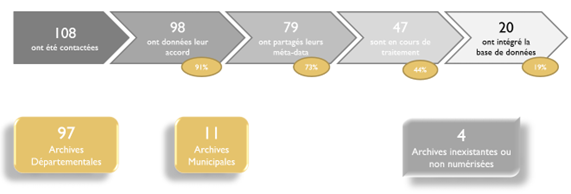
\includegraphics[width=0.9\linewidth]{Figures/Partie 1/Fig.1.2 - Participation des services d'archives.png}
        \caption[Participation des services d'archives]{Participation des services d'archives}
        \label{fig:Fig1.2}
    \end{figure}

Parmi les 20 services ayant décliné, les raisons sont multiples : pour certains, les fichiers n'ont pas encore été numérisés, ou pas en totalit, pour d'autres, les archives ont disparues. Enfin, certains n'ont pas encore répondu ou ont refusé de participer (seulement un service jusqu'ici).

SocFace demande aux services d’archives de verser les images ainsi qu’un fichier comprenant les métadonnées qui leur sont associées. Sur les 98 services d’archives ayant accepté le projet, 79 ont déjà envoyé ces fichiers, parfois avec des informations manquantes. Il faut également noter que certaines années ou communes sont manquantes, pour diverses raisons. A ce jour, la collecte d’image se chiffre à 10 557 555. La projection finale est à 15 millions d’images, ce qui représente un stockage de 3 Téra octets. Voici un tableau comparatif\footnote{Ressources utilisées pour la création du tableau : \\ 
\href{https://ischoolonline.berkeley.edu/blog/big-data-infographic/}{https://ischoolonline.berkeley.edu/blog/big-data-infographic/}\\ 
\href{https://www.bnf.fr/fr/la-bnf-en-chiffres}{https://www.bnf.fr/fr/la-bnf-en-chiffres}\\
\href{https://www.teradata.fr/glossary/what-is-an-exabyte}{https://www.teradata.fr/glossary/what-is-an-exabyte}
}, pour comprendre l'ampleur que cela représente  :  

\renewcommand{\arraystretch}{1.5}

    \begin{table}[H]
    \centering
    \begin{tabular}{p{12cm}c}
        \toprule
        \textbf{Institution} & \textbf{Stockage} \\ % Première ligne en gras
        \midrule
        Œuvre Complète de Shakespeare & 5 mégaoctets \\
        Ensemble des enregistrements de Beethoven & 20 gigaoctets \\
        Collection des imprimés de la librairie du Congrès (USA) & 10 téraoctets \\
        Ensemble des collections de la BnF & 2000 téraoctets \\
        Totalité des ouvrages écrits depuis le début de l’humanité & 50 pétaoctets \\
        Totalité des mots prononcés depuis le début de l'humanité & 5 pétaoctects \\
        \bottomrule
    \end{tabular}
    \caption{Comparaison des volumes de stockage pour différentes collections}
    \label{tab:stockage}
\end{table}

Pour rappel :

\begin{table}[H]
    \centering
    \begin{tabular}{|c|c|}
        \hline
        \textbf{Unité} & \textbf{Valeur en Octets} \\
        \hline
        1 Octet & 1 \\
        1 Kilooctet (Ko) & 1{,}024 \\
        1 Mégaoctet (Mo) & 1{,}048{,}576 \\
        1 Gigaoctet (Go) & 1{,}073{,}741{,}824 \\
        1 Téraoctet (To) & 1{,}099{,}511{,}627{,}776 \\
        1 Pétaoctet (Po) & 1{,}125{,}899{,}906{,}842{,}624 \\
        1 Exaoctet (Eo) & 1{,}152{,}921{,}504{,}600{,}000 \\
        \hline
    \end{tabular}
    \caption{Correspondances des unités de volumes}
    \label{tab:volumes}
    \end{table}
    
    \section{Peut-on parler de \textit{Big Data?}}

Au vu des projections établies en début de projet, le nombre de données collectées est considérable. Il faut donc poser la question : peut-on parler de Big Data ? Christophe Brasseur, auteur de \textit{Enjeux et usages du Big Data} \cite{brasseurEnjeuxUsagesBig2016} donne cette définition : 
    \begin{quote}
    \textit{"Le Big Data représente d’énormes volumes de données, structurées ou non structurées, difficilement gérables avec des solutions classiques de stockage et de traitement, qui proviennent de sources diverses et sont produites en temps réel."}
    \end{quote}
Cette définition est intéressante car elle donne quelques conditions d’identifications de la big data, mais elle reste assez vague. L’article \textit{Et demain ? Archivage et Big Data} \cite{charaudeauDemainArchivageBig2015}donne la règle des trois V, issue d’articles anglo-saxons\footnote{Certains articles ajoutent un quatrième V, pour "véracité"} :

    \begin{itemize}[label=\textbullet] % Change les puces en points noirs
    \item \textbf{Volume} : on parle de quantité « considérable », mais qui doit être prise en compte dans un contexte. Il n’y a aucun seuil prédéterminé au-delà duquel on pourrait parler de big data.
    \item \textbf{Variété} : cela implique différents types de données (structurées ou non-structurées) qui proviennent de sources différentes. Elles sont alimentées régulièrement, ce ne sont donc pas des données figées.
    \item \textbf{Vélocité} : ce terme illustre le fait que les données sont générées et collectées dans un « délai de temps fortement réduit ». Encore une fois, il n’y a pas ici de vitesse prédéterminée.
\end{itemize}

En partant de ces définitions, peut-on qualifier les données traitées dans le cadre du projet SocFace de « Big Data » ? Si l’on suit Christophe Brasseur, le début de la définition correspond. Nous parlons d’un volume extrêmement important, qui se compte en téraoctets. Cependant – et c’est un problème dans la règle des trois V – il n’y a pas de variété des sources. Si les images issues des archives proviennent de services différents, le processus pour la création des données à partir de ces images est identique. Par ailleurs, on ne peut pas dire que les données sont produites en temps réel puisqu’il n'y a pas d’automatisation de la production de données. Les départements sont traités petit à petit, et les problèmes techniques peuvent ralentir chaque processus. Même dans l’hypothèse où cette automatisation est mise en place dans le futur, l’alimentation finira par se tarir. De fait, il n’y a qu’un nombre déterminé de listes de recensement sur la période. \\
 Le projet ne peut pas être considéré comme faisant partie du phénomène "big data" stricto sensu. Mais l'importance des données est telle qu'elle nécessite la création d'outils \textit{ad hoc}. L'utilisation seule n'est pas possible, il faut une mise à l'échelle. En cela, ce projet se rapproche du big data. \\
 
 La dimension de ces données est au cœur du projet et constitue l'un de ses objectifs principaux. Cela explique pourquoi le projet nécessite la collaboration de différents acteurs aux compétences variées. En conséquence, il s'agit d'un projet interdisciplinaire dont l'organisation et la coordination doivent être clairement comprises. 
\chapter{Entre interdisciplinarité et collaboration}
Le projet SocFace est porté par plusieurs acteurs : l'\gls{INED}, PSE, le SIAF, et Teklia.Au-delà de la diversité de ces institutions, de leurs statuts et de leurs missions, ce projet illustre l’importance de l’interdisciplinarité dans la recherche. Plus spécifiquement, pour SocFace, il est intéressant d’étudier la dynamique entre des institutions de la recherche publique coopérant avec Teklia, entreprise privée. 

    \section{Les acteurs du projet}

Le projet SocFace implique plusieurs acteurs aux rôles divers. Les deux principales entités dirigeantes sont l'{\gls{INED}} et Teklia, tandis que le \gls{SIAF} et \gls{PSE} interviennent à certaines étapes du projet.\\
l'\gls{INED} est un Établissement Public à Caractère Scientifique et Technologique (EPST). Les sujets couverts par les chercheurs sont très larges : démographie, genre, sexualité, migrations, familles etc… Ces chercheurs ont des profils très divers : démographes, statisticiens, ingénieurs informatiques, sociologues ou historiens. Le projet est initié par Lionel Kesztenbaum, responsable de l’unité Histoire et Populations. Il n’y a pas d’équipe dédiée au projet à temps plein, mais une doctorante, un chercheur associé et parfois des stagiaires. D’autres chercheurs interviennent ponctuellement. Les équipes de l'\gls{INED} apportent leur expertise en sciences sociales. Il faut cependant noter que la plupart ont aussi des compétences en traitement et gestion de bases de données.\\
Teklia est une société fondée en 2014 par Christopher Kermorvant. Elle se spécialise sur le traitement automatique en langage naturel et la reconnaissance optique de caractère, ce qui est à la base du projet SocFace. En utilisant la technologie du \gls{DL} et de l’intelligence artificielle, Teklia permet la conversion de documents en données structurées, interrogeables dans une base de données. Ces solutions s’adressent à des entreprises, des industriels ou institutions publiques. Le projet SocFace s’inscrit dans leurs projets en Recherche et Développement (R\&D). SocFace n’est d’ailleurs qu’un projet parmi d’autres, car Teklia s’est associé à de nombreux partenaires publics dans la sauvegarde du patrimoine public. On peut citer les Archives Nationales, l’Institut de la Recherche et d’Histoire des Textes (IRHT), ou la National Norwegian Library. Les équipes de Teklia dédiées à SocFace sont composées d’ingénieurs informatiques, ingénieurs réseaux et architectes, qui mettent au point les logiciels et programmes nécessaires à la réalisation du projet. 
Paris School of Economics est une institution de recherche fondée en 2006 par le CNRS, l’école des Ponts, \gls{PSL}, Paris 1, l'\gls{ENS} et l’\gls{EHESS}. L’objectif est de créer une communauté de chercheurs et d’enseignants au service des questions économiques, dans différents domaines. C’est un établissement qui prône l‘interdisciplinarité et cherche à faire travailler ensemble chercheurs en sciences sociales et économiques ou ingénieurs. L’un des objectifs de SocFace est justement de pouvoir améliorer la recherche historique et économique de la France sur la période. L’un des chercheurs associé au projet, Jérôme Bourdieu, a d’ailleurs déjà participé à une précédente enquête avec Lionel Kesztenbaum : L’enquête TRA, qui s’intéressait déjà la population française au XIXe siècle.\\
Enfin, le projet est porté par le SIAF. Ce service permet la coordination des différentes archives municipales, départementales et nationales. Il est chargé de faire appliquer des politiques communes concernant les archives. Concernant SocFace, c’est bien l'\gls{INED} et Teklia qui contactent ces services mais le \gls{SIAF} a permis la publicisation au début du projet. Il intervient en cas de blocage ou de lenteur dans les échanges et est un point de contact essentiel pour les services d'archives. La base de données pourra être consultée par ceux qui viennent consulter les Archives, faisant gagner un temps considérable aux usagers. Les services d’archives ont donc tout intérêt à participer au projet, mais cela peut parfois représenter un surcroit de travail important. De fait, tous les services n’avaient pas nécessairement numérisé les listes de recensement avant le début du projet.\\
Ajoutons que le projet est financé par l’ANR, l’Agence Nationale pour la Recherche, ce qui est bien entendu un gage de qualité, mais démontre aussi que le projet a dû respecter un certain nombre de conditions et est fortement attendu dans ses résultats.\\

Ainsi, nous avons vu qui étaient les équipes derrière le projet SocFace. Leur parcours dans la recherche diffère car il y a d’un côté des instituts de recherche classique, comme l'\gls{INED} et \gls{PSE}, et de l’autre des structures pour qui la recherche est seulement une partie de leurs activités. Mais une autre dichotomie traverse ces équipes : le secteur public collabore ici avec une entreprise privée. 
    
    \section{Les avantages du partenariat entre le public et le privé}

De fait, comme beaucoup de projet de recherche, SocFace associe public et privé. Ce type de partenariats n’est pas rare, même si on le retrouve davantage dans les projets de sciences dures comme la médecine ou la chimie. Selon la publication \textit{État de l’Enseignement supérieur, de la Recherche et de l’Innovation en France n°12}, on distingue trois types de partenariats dans la recherche : 

    \begin{itemize}[label=\textbullet] % Change les puces en points noirs
    \item \textbf{La recherche contractuelle},qui implique un commanditaire privé sous-traitant des travaux de Recherche \& Développement (R\&D) à une université ou un laboratoire. Cela représente 5,2\% de la recherche
    \item \textbf{La recherche collaborative}, qui permet l’association d’une entreprise privée avec un laboratoire et dans laquelle les coûts et les résultats sont partagés. 
    \item \textbf{Les travaux de consultance} dans lesquels un.e chercheur.se partage sa parole d’expert.e auprès d’une entreprise privée. 
\end{itemize}

En l’espèce, les acteurs de SocFace se situent dans la deuxième catégorie : les acteurs sont à égalité dans la responsabilité du projet et travaillent ensemble au quotidien. Ce type de recherche est choisi par 17\% des entreprises technologiquement innovantes, et le chiffre est en hausse. Elle est également davantage prisée par les grandes entreprises (plus de 250 salariés), ce qui n’est pas le cas de Teklia. De même, les entreprises coopèrent davantage avec les universités ou les établissements d’enseignements supérieurs. En l’espèce,l’\gls{INED} et \gls{PSE} ne sont pas des établissements d'enseignement supérieurs mais des instituts de recherche. Ce cas de figure représente 11\% des configurations. SocFace n’est donc pas un projet typique des partenariats publics/privés, mais s’inscrit malgré tout dans une tendance grandissante de la recherche, qui encourage les partenariats.

On ne parle pas ici de PPP (Partenariats Public-Privé) qui désigne plus généralement des marchés de partenariats, particulièrement dans le secteur hospitalier ou de la construction. Mais il est intéressant de comprendre la dynamique de travail entre une entreprise privée et des institutions publiques - en dehors de tout cadre administratif. Dans un article intitulé \textit{Le concept de "partenariat public" est-il bien posé ? la coresponsabilité de l’économie privée en politique de développement}\footnote{\fullcite{ulrichConceptPartenariatPublicprive2005a}}, Peter Ulrich et Florien Wettstein, deux chercheurs en science économique de l’Université de Saint-Gall, questionnent ce concept. Selon eux, des « présupposés normatifs » persistent : le secteur privé apporterait au secteur public cette efficacité qui lui manque nécessairement. Et ainsi, le privé serait indispensable aux institutions publiques qui ne pourraient pas avancer sans cela. A l’inverse, certains pourraient « diaboliser » le secteur privé, qui, seulement intéressé par la productivité, ne ferait pas bon ménage avec le rythme de la recherche. Pour autant, il semble évident qu’il est nécessaire de nuancer ces vues que l’on pourrait qualifier de caricaturales. L’exemple de SocFace est intéressant pour cela. L’initiative du projet est conjointe : en effet, Teklia et l’\gls{INED} travaillaient tous deux sur un projet similaire à présenter à l’ANR et ont décidés de s’associer avant d’en soumettre deux différents. On voit donc que l’initiative est partagée. 
On peut toutefois noter des différences, plus matérielles. Ainsi, l’\gls{INED} connait une gestion de la sécurité des serveurs plus stricte que ne peux le faire Teklia, qui est une plus petite structure et peut se permettre d’être plus souple. Par ailleurs, si le financement du projet se fait globalement par le biais de l’ANR, il faut noter que Teklia est une société privée, qui vend des solutions à des clients. Si l’objectif de l’\gls{INED} est bien la recherche, pour Teklia, le R\&D n’est qu’une partie de l’ensemble des activités.\\

Cette différence public/privé n’est donc pas une opposition mais une véritable complémentarité. Les équipes doivent collaborer. Mais n’appartenant pas aux mêmes secteurs de la recherche (les sciences sociales et la technologie), on peut parler d’une collaboration interdisciplinaire. A quel type d’interdisciplinarité se réfère-t-on ?

    \section{La collaboration des équipes, au-delà de l'interdisciplinarité}

Nous avons vu que les différents acteurs du projet SocFace étaient hétérogènes dans leur nature et leurs compétences et collaboraient pourtant. Plusieurs notions se recoupent pour définir le travail commun entre différentes institutions : interdisciplinarité, transdisciplinarité et pluridisciplinarité. A laquelle peut-on rattacher le projet SocFace ?\\

Le premier concept à être apparu est la pluridisciplinarité. 

\begin{quote} 
    \textit{"Elle peut être entendue comme une association de disciplines qui concourent à une réalisation commune, mais sans que chaque discipline ait à modifier sensiblement sa propre vision des choses et ses propres méthodes. À ce titre, la pluridisciplinarité existe depuis longtemps, même si son importance s'est accrue de nos jours."}\footnote{\fullcite{DefMulti}}
\end{quote}
Ce concept rassemble donc plusieurs disciplines, qui vont collaborer mais en restant chacune dans leur zone de compétence, sans réellement dialoguer entre elles. Les analyses des uns ne vont pas nécessairement interférer sur les résultats des autres. On pourrait comparer cette méthode de travail à la scolastique du Moyen-Âge, où les sept arts libéraux étaient associés à l’université.\\ 
L’interdisciplinarité est le degré supérieur de la collaboration, selon Pierre Delattre. Davantage qu’une simple discussion entre disciplines, on recherche ici à intégrer les concepts et les méthodes d’une autre discipline dans son travail. L’approche est plus générale, avec un entrecroisement des disciplines et une véritable interaction. Si les collaborations multidisciplinaires sont motivées par un sujet d’études commun, l’interdisciplinarité n’a pas seulement le sujet d’étude au centre de ses préoccupations : elle cherche à explorer les analyses, les perspectives, les résultats de chacune des disciplines concernées. Il n’y a pas de juxtaposition du travail de chacun, mais une véritable comparaison, et le travail des uns vient enrichir le travail des autres pour le faire avancer. Aujourd’hui, le domaine de la recherche est cloisonné : sciences dures ou sciences humaines, histoire ou géographie, médecine ou physique etc…  Pour autant, cette façon de travailler remonte à la nuit des temps : les philosophes grecs étaient astronome et mathématiciens, Léonard de Vinci concevait des armes de guerres et s’adonnait à la dissection, Vauban a construit des forteresses et écrit des traités de fiscalité. Le XX\textsuperscript{e} siècle, dans le sillage du siècle précédent, a vu les domaines de la recherche et de l’enseignement se démocratiser et s’élargir. Mais dans le même temps, les disciplines ont eu tendance à s’isoler les unes des autres, à se spécialiser. Selon Sandrine Louvel dans son article \textit{Ce que l’interdisciplinarité fait aux disciplines} \footnote{\fullcite{louvelCeQueInterdisciplinarite2015}}, la transition vers une meilleure coopération entre chercheurs commence vers la fin des années 60 et \textit{"trouve son apogée pendant les années 90"}. Cette impulsion est avant tout politique, et se traduit par le fait de favoriser les projets mettant en jeu plusieurs disciplines. Au-delà des disciplines, c’est le projet et les réponses apportées qui importent.\\ 
Enfin, la transdisciplinarité va encore plus loin, en cherchant à intégrer non seulement d’autres disciplines universitaires mais également des acteurs non académiciens. Le champ des collaborateurs travaillant sur un projet est élargi. Par exemple, on peut faire intervenir le personnel politique, une association, un groupe déterminé. Les théoriciens de la transdisciplinarité sont partis du constat que les problèmes contemporains, plus complexes selon eux, nécessitaient une réponse différente de ce que la recherche pouvait jusque là proposer.\\

De quelle notion relève SocFace? Selon les définitions données, on penche pour l’interdisciplinarité. De fait, la collaboration entre les différentes équipes du projet est étroite comme nous allons le voir. Par ailleurs, ces acteurs possèdent des compétences différentes : informaticien, ingénieur, historien, sociologue, démographe. Enfin, concernant la nature des acteurs : Teklia n’est pas un acteur académique au sens propre du terme. Dans un article sur l’interdisciplinarité dans les humanités numériques\footnote{\fullcite{benelQuelleInterdisciplinaritePour2014}}, Aurélien Bénel explique : 
\begin{quote}
\textit{"Ni l’usage d’un blog en histoire, ni la réalisation d’une base de données en littérature ne sont des projets interdisciplinaires. L’embauche d’un « informaticien » n’y change rien. L’interdisciplinarité nécessite un statut équivalent des représentants des disciplines, un respect de l’autre comme exerçant une discipline scientifique de plein droit. Quand une discipline est éclipsée par ses productions auprès du grand public, l’autre discipline ne doit pas l’enfermer dans ce qu’elle attend de ses productions, mais lui laisser la latitude d’innover. Ce besoin d’innovation signifie aussi qu’un type de projet, comme l’encodage savant de textes avec des balises, peut avoir été interdisciplinaire en 1987 et ne plus l’être aujourd’hui".}
\end{quote}
Cet article a été écrit en 2014 et illustre l’évolution de la notion d’interdisciplinarité mais aussi des humanités numériques jusqu’ici. Pour le projet SocFace, on ne parle pas d’"informaticiens" mais bien d’ingénieurs informatiques, de développeurs, d’architectes de la donnée. L’innovation – et donc la recherche - est au cœur du développement de l’entreprise. Les articles rédigés par les équipes de SocFace, destinés à des publications scientifiques, sont signés par des membres de Teklia, de l’\gls{INED},du \gls{SIAF} et de \gls{PSE}. Il y a une véritable reconnaissance de la compétence et de l’expertise de ces spécialistes du numériques. Cela ne veut pas dire pour autant que les chercheurs en sciences sociales du projet sont dépourvus de toute connaissance dans ce domaine. Ainsi, Lionel Kesztenbaum maitrise parfaitement les outils de gestion d’une base de données, et Christopher Kermorvan travaille depuis 10 ans avec des services d'archives. Cela permet un dialogue constant des équipes.\\

On voit donc que les acteurs du projet, bien que venant d’horizons différents, s’accordent autour d’un objectif commun. C’est la définition de l’interdisciplinarité : la collaboration entre plusieurs disciplines différentes et complémentaires. Si la collaboration ne se fait pas toujours dans l’interdisciplinarité, c’est bien le cas ici. C’est pourquoi il faut trouver des façons de travailler ensemble et se répartir les différentes étapes du projet, selon les compétences de chacun. 
\chapter{Mettre en place un processus qui intègre l’ensemble des acteurs}
On parle ici d’un projet nécessitant recherche et développement technologique. Aussi, la recherche vient alimenter le développement, qui s’adapte aux besoins de la recherche. Plusieurs outils sont partagés par les différentes équipes : d’une part les outils développés par Teklia qui permettent l’extraction et la lecture \gls{HTR}, et d’autre part, des outils plus simples pour la gestion du projet.  

    \section{Une chaîne de traitement intégrée}

SocFace est un projet où la technologie joue un rôle clef. Il est donc nécessaire d’assurer un processus de traitement (workflow). La chaîne de traitement concerne la production de la base de données\footnote{Voir Annexe A}. 

\begin{figure}[H]
        \centering
        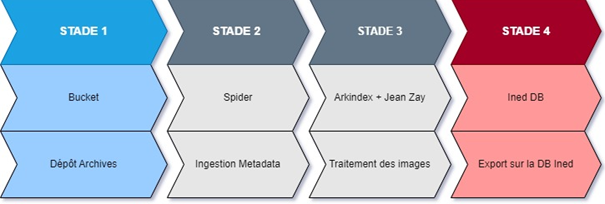
\includegraphics[width=1.0\linewidth]{Figures/Partie 1/Fig.1.3 - Extrait du panorama général des process.png}
        \caption[Extrait du panorama général des process]{Extrait du panorama général des process}
        \label{fig:Fig1.3}
    \end{figure}

Ce processus commence avec les services d’archives. Ils sont contactés par SocFace, qui leur propose de participer au projet. Comme on l’a dit, le taux de réponse est plutôt positif. Lorsque les services d'archives sont prêtes, elles donnent les listes de recensement sous forme d’images \gls{IIIF}\footnote{Voir Glossaire}, ainsi qu’un fichier qui contient les métadonnées associées aux images. Elles peuvent livrer un disque dur, ou bien se connecter sur les serveurs de Teklia. Il faut ajouter que parfois, les services d’archives utilisent une solution externe, comme Naoned. Plusieurs sont dans ce cas, c’est pourquoi les équipes du projet se sont rapprochées directement de ces fournisseurs de solutions pour regrouper les transferts de fichiers. Cette étape du processus peut prendre beaucoup de temps, soit parce que les images n’ont pas été encore numérisées, soit parce que des problèmes techniques ralentissent le transfert. De fait, tous les services d’archives n’ont pas les mêmes moyens humains, ni le même niveau d’expertise concernant ces questions. Ces échanges sont assurés par des équipes de l’INED ou parfois par Teklia, lorsque des questions plus précises sur les serveurs sont abordées. Si les services semblent hésiter, l’aide du SIAF est demandée. 

\begin{figure}[H]
        \centering
        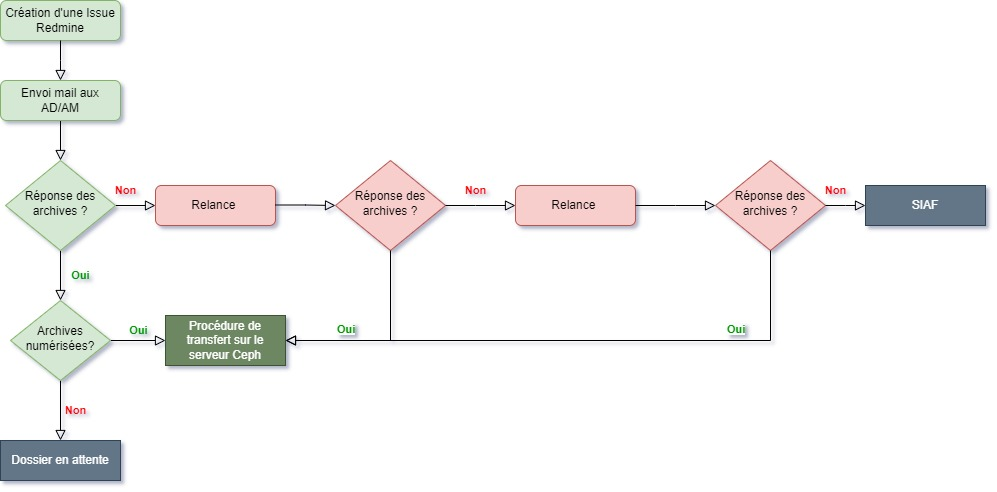
\includegraphics[width=0.8\linewidth]{Figures/Partie 1/Fig.1.4 - Contact Archives .jpg}
        \caption[Processus de contact des archives]{Processus de contact des archives}
        \label{fig:Fig1.4}
    \end{figure}

Une fois les données reçues, le travail sur l’image commence. Les images livrées par les services d’archives sont téléchargées dans l’outil \Spider{}. Une fois associées à leurs métadonnées, elles sont exportées ensuite sur l’outil \Arkindex{}, qui va opérer la magie de l’\gls{HTR} : reconnaissance et classification des pages, reconnaissance des \gls{entités} et regroupement en foyer (\textit{\gls{households}})\footnote{Voir Glossaire}, puis export de ces informations dans la base de données de l’INED. Ces différentes étapes sont assurées par les équipes de Teklia, qui possèdent la compétence informatique. Ces outils ont d’ailleurs été conçus par Teklia. Le process tel qu’il est décrit ici parait très simple, mais les spécificités techniques nécessitent en réalité de constants ajustements.

    \section{Les différents outils utilisés pour le projet}

Afin de bien comprendre l’ampleur de SocFace, il faut commencer par comprendre les outils utilisés par l’ensemble des équipes. Ces outils ont été développés pour la plupart par Teklia, qui en assure également la gestion quotidienne.

        \subsection{SPIDER}

Cet outil\footnote{Voir Annexe D} permet d’associer les images, généralement en .jpeg, avec un fichier de métadonnées également fourni par les archives, sous format .xml ou .csv (si le fichier est en .xml, il est nécessaire de le convertir en .csv via un script Python). Ces métadonnées identifient dans chacune des images : la commune et l’année. Parfois, il y a un chemin \gls{ARK}\footnote{Voir Glossaire}, ce qui permet de retrouver les images beaucoup plus facilement.  
L’outil \Spider{} est connecté aux serveurs contenant les images. Ces serveurs sont également gérés par Teklia. Il est souvent nécessaire de recommencer le traitement plusieurs fois, et même dans ce cas, on peut avoir des erreurs. Cela dépend beaucoup de la qualité du fichier de métadonnées fournit par les Archives. Ceux-ci sont en effet très hétérogènes. On aurait pu penser que fournir un modèle à suivre pour la fourniture des métadonnées aurait été plus utile pour le projet. Mais cela se serait révélé en réalité contre-productif : les services d’archives auraient pu remettre leur participation en question s’il avait fallu adapter leurs propres fichiers. 
Une fois les images associées entre elles, elles sont envoyées sur l’outil \Arkindex{}.

\begin{figure}[H]
        \centering
        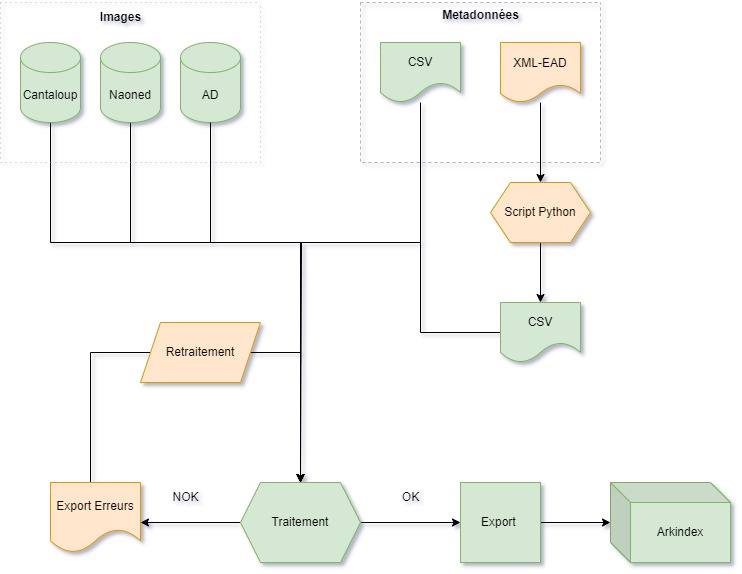
\includegraphics[width=0.8\linewidth]{Figures/Partie 1/Fig.1.5 - Processus Spider.jpg}
        \caption[Processus de l'outil \Spider{}]{Processus de l'outil \Spider{}}
        \label{fig:Fig1.5}
    \end{figure}

        \subsection{ARKINDEX}

\Arkindex{}\footnote{Voir Annexe C} est l'outil principal de Teklia qui permet de convertir les images numérisées en texte, de reconnaître les \gls{entités}\footnote{Voir Glossaire}, et d'exporter ces données vers une base de données.

\begin{figure}[H]
        \centering
        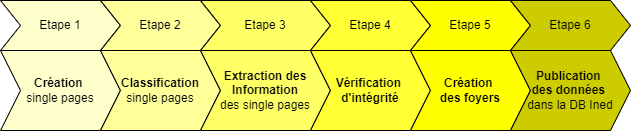
\includegraphics[width=0.8\linewidth]{Figures/Partie 1/Fig.1.6 - Arkindex General.png}
        \caption[Processus de l'outil \Arkindex{} (Général)]{Processus de l'outil \Arkindex{} (Général)}
        \label{fig:Fig1.6}
    \end{figure}

Avant de pouvoir lire et extraire les informations des images numérisées et les exporter dans la base de données, il faut travailler sur les pages. Les listes de recensement sont contenues dans de grands registres : il faut s’assurer que chaque page est traitée indépendamment de la page suivante, ce qui serait une double page. La technologie détecte donc naturellement une double page, mais l’outil va les découper pour créer des \gls{SP}\footnote{Voir Glossaire}, beaucoup plus facile à traiter. 
Une fois les pages découpées, elles sont classifiées : la machine identifie les premières pages, les dernières pages et les pages intermédiaires. Pour cela, elle est entraînée via des modèles : on lui donne des images déjà classifiées pour lui apprendre à reconnaître les types de pages et le modèle est ensuite appliqué aux images des archives via des workers¸c’est-à-dire des scripts qui tournent en arrière-plan. 
Le cœur de l'\gls{HTR} commence ensuite : en utilisant des modèles entrainés, les images sont analysées, et les informations extraites. Ces modèles n’ont pas été créés par Teklia, mais récupérés en Open Source. Les deux principaux sont \gls{DAN} et \gls{YOLO}. \YOLO{} a été créé par Joseph Redmon en 2016.  C’est un algorithme de détection d'objets en temps réel qui analyse une image en une seule passe pour identifier et localiser les objets. L’algorithme divise la page en plusieurs boites et effectue des prédictions en fonction de la façon dont il a été entraîné. Son avantage est qu’il travaille sur toutes les cases en même temps, là où les précédents modèles avaient besoin de repasser plusieurs fois sur la page. \DAN{}\footnote{Pour plus d'informations, cf le \href{https://github.com/FactoDeepLearning/DAN}{GitHub} du projet} a été créé par Denis Coqueret et est également orienté sur la reconnaissance manuscrite, et l’extraction d’information. 
Ces modèles doivent être entraînés pour fonctionner sur les images des archives. Il faut donc les nourrir avec des images déjà analysées et indexées. Pour cela, Teklia a créé Callico, qui permet de lancer des campagnes d’indexation. En faisant appel à des volontaires ou des étudiants rémunérés, des centaines de pages sont traitées correctement, avec détection manuelle des zones, et indexation du texte. Ces pages sont ensuite intégrées au modèle, qui peut dès lors prédire des pages non traitées en fonction des informations qu’il a apprises. C’est l’utilisation du \gls{DL} pour la reconnaissance manuscrite : on entraîne la machine à apprendre à détecter les informations pour qu'elle finisse par les reconnaître sans entraînement. Cela nécessite un nombre considérable de données d’entraînements : plus la machine apprend, plus elle devient experte. Ces outils sont très efficaces pour l'extraction des mentions simples comme les noms ou les dates, mais connaissent des difficultés avec les adresses. De fait, celles-ci sont souvent orientées verticalement, contrairement aux autres informations. Il faut donc apprendre aux modèles à orienter leur lecture différemment. 
Il faut noter que ces outils fonctionnent grâce au serveur JeanZay, le supercalculateur du CNRS\footnote{Voir Chapitre 6}.

        \subsection{Metabase}
Une fois les données identifiées et extraites, elles sont exportées vers une base de données, hébergée par l’\gls{INED}. A cause de l’ampleur du projet, cette base de données est difficilement accessible et exploitable sans un programme adapté, en l’espèce, R. Il est difficile de naviguer dans cette base de données sans connaissances préalable, c’est pourquoi il a fallu trouver une autre solution d'accès. Le choix s’est porté sur Metabase\footnote{https://www.metabase.com/}, qui est accessible en OpenSource.\\

On voit donc que ce projet nécessite des outils exigeants, qui demandent un travail constant et poussé, mais qui peuvent également réaliser un travail puissant et de qualité. Leur articulation est fragile, et le process dans son ensemble prend un certain temps. Au-delà des outils développés par les ingénieurs informatiques de Teklia, qui agissent sur la donnée elle-même, on doit également mentionner les outils de gestions du projet, qui aident à la collaboration entre les équipes.  

    \section{Les outils de gestion}

Comme on l'a vu précédemment les différents outils sont utilisés par plusieurs équipes : L’\gls{INED}, Teklia et parfois le \gls{SIAF}. Le processus de production est majoritairement opéré par les équipes de Teklia, mais tout se fait en concertation avec l’INED. De même, le SIAF intervient lorsque des difficultés ou des lenteurs interviennent avec les services d’archives. Or, toutes ces équipes ne sont pas géographiquement dans les mêmes lieux. Teklia possède des bureaux parisiens mais une partie de leurs collaborateurs sont en région. Et bien entendu, les autres institutions sont chacune dans leurs locaux. Il faut donc s’entourer – dès le début du projet - d’outils de gestion de projet qui permettent d’assurer une fluidité dans les échanges et une entraide entre les membres des différentes équipes.\\ 
On utilise généralement la méthode \gls{AGILE}\footnote{Voir Glossaire} pour améliorer les échanges dans les projets informatique. SocFace est un projet hybride, avec du développement, mais aussi de la recherche. Dès lors, on retrouve quelques notions propres à AGILE, comme le découpage du projet en phase avec des itérations régulières : on avance petit à petit, dans les différentes composantes du projet. 

            \subsection{REDMINE}

REDMINE est un outil de gestion de projets, qui permet de créer des \textit{"issues"}, c’est-à-dire des tâches, chacune assignées à des \textit{"projets"}. Cet outil est primordial, en raison de l’ampleur du projet. Comme on l’a vu, il y a plusieurs phases et chacune correspond à un "projet". Elles sont concomitantes : on n'attent pas qu’une phase soit terminée pour commencer la suivante :

\begin{itemize}[label=\textbullet] % Change les puces en points noirs
    \item La collecte auprès des archives départementales ou municipales 
    \item Les campagnes d’annotations des volontaires
    \item L’entraînement des modèles 
    \item La production 
    \item La création de la base de données 
    \item L'appariement (linking)
\end{itemize}

Sur chacun de ces \textit{"projets"}, les équipes créent des tâches qui peuvent être assignés à n’importe quel membre et visible de tous les autres, qui peuvent également ajouter des commentaires. Cela permet de garder un historique complet des problèmes éventuellement rencontrés et des solutions trouvées. 
A noter qu’il existe également des GitLab, alimentés à la fois par les équipes de l’INED et de Teklia, qui permet de documenter les process et les technologies utilisées ainsi qu'un wiki commun. Ce point est essentiel pour permettre à chaque membre du projet de travailler en autonomie.

        \subsection{Les réunions}

Afin de favoriser la collaboration entre toutes les équipes, des réunions hebdomadaires sont mises en place entre l’INED, Teklia et PSE. Cela permet de faire un point sur l'avancement du projet, sur les questions et les nouvelles tâches à venir. Il y a également des réunions régulières avec le SIAF. Bien entendu, chacune des équipes organise aussi ses propres réunions. Il faut également noter l’utilisation d'un logiciel de discussion, afin de favoriser le dialogue entre les équipes.\\ 
Tous ces outils sont bien entendu utilisés pour la majorité des projets - de recherche ou non, informatiques ou non. Mais ici, la singularité est qu’il s’agit d’institutions différentes, donc avec des contraintes différentes, du matériel différent, un personnel différent. Ces outils sont utiles pour fluidifier le travail mais aussi pour assurer un bon dialogue et une communion entre des équipes qui n’étaient pas destinées à travailler ensemble : chacune des équipes doit apprendre à travailler avec le matériel de l’autre, à utiliser le vocabulaire de l’autre. Cela nécessite une adaptation. Car si on parle ici de collaboration, comme dans un projet classique, il s’agit aussi d’interdisciplinarité. Un chercheur en sociologie doit donc pouvoir comprendre le langage d’un ingénieur informatique qui lui doit pouvoir comprendre les besoins d’un démographe. Le fait de garder une trace écrite, dans le logiciel Redmine, mais aussi les comptes-rendus des réunions, permet de faciliter ce dialogue entre des disciplines et donc des compétences difficiles. Cette mise en place est primordiale pour des projets de cette envergure, afin d’éviter les erreurs de communication, ou des malentendus. D’autant plus que la très grande majorité du personnel travaillant sur le projet est en télétravail, ce qui limite les possibilités de régler les problèmes rapidement. \\
Le travail d’équipe nécessite donc la mise en place d’outil de travails communs, d’autant plus que ces équipes sont dispersées sur plusieurs sites, et appartiennent à des structures différentes.\\ 

Le projet SocFace incarne donc un exemple ambitieux d’interdisciplinarité, entre la recherche académique et numérique. Cela illustre également la manière dont les associations entre le public et le privé peuvent dynamiser la recherche et l’innovation. À travers l’étude de cette coopération interdisciplinaire, nous avons observé que loin d’être en opposition, ces deux secteurs se complètent en apportant chacun leur expertise spécifique. Cette complémentarité s’est révélée essentielle dans le développement des outils technologiques qui sous-tendent SocFace, tout en répondant aux exigences rigoureuses du domaine de la recherche scientifique. Après avoir analysé les fondements de ce partenariat, il est désormais important d’examiner la manière dont les données, sont gérées et valorisées. Nous allons donc examiner les défis liés à la collecte, l’intégration et l’analyse des données publiques. Ces données, souvent fragmentées et hétérogènes, nécessitent des méthodes innovantes pour en extraire toute leur richesse. Nous explorerons comment SocFace parvient à transformer ces informations brutes en connaissances exploitables, tout en assurant leur protection et leur intégrité.
	
	\part{Les données perdues dans l'interdisciplinarité}
 
L'un des éléments crucial pour le succès du projet SocFace est la gestion efficace et la valorisation des données collectées. En effet, les données constituent la base sur laquelle repose l'ensemble des analyses et des résultats attendus. Ce chapitre se propose d'explorer les diverses étapes et techniques mises en œuvre pour assurer la qualité, la cohérence et l'intégrité des données, de leur extraction à leur intégration dans la base de données. Dans un premier temps, nous examinerons les méthodes de collecte et d'intégration des données, en mettant en lumière les particularités des sources utilisées et les contraintes techniques auxquelles les équipes ont dû faire face. Nous verrons ensuite un outil particulier, Metabase, qui permet la visualisation des données. Enfin, nous aborderons la question de la sécurisation et de la fiabilité des données, un aspect fondamental pour garantir la l'intégrité des informations manipulées tout au long du projet. Ainsi, ce chapitre permettra de comprendre comment le projet SocFace transforme un ensemble de données hétérogènes en une base de connaissances structurée et utilisable pour la recherche.
\vspace*{\fill}
\begin{center}
  % Ajouter un joli cadre autour de l'image
  \setlength{\fboxsep}{5pt}  % Espace entre l'image et le cadre
  \setlength{\fboxrule}{1pt} % Épaisseur du cadre
  \fbox{
    
\includegraphics[width=0.8\textwidth]{Figures/Partie 2/Illus.Partie 2.png}}\\
    \vspace{0.5em} % Espace entre l'image et la légende
    {\scriptsize \textit{Crédit : Datactivist.}}
\end{center}

 \chapter{L’impact d’un projet aux acteurs multiples sur l’intégrité des données}

La donnée occupe une place centrale dans le projet, à la fois comme objectif ultime et comme matière première de toute la chaîne de traitement. Il est donc essentiel de saisir sa nature et son rôle à chaque étape du projet. Comprendre la nature des données conduit inévitablement à s'interroger sur leur statut juridique : à qui appartiennent-elles et comment s’inscrivent-elles dans le cadre légal des archives ? Par la suite, nous examinerons le parcours des données, manipulées par diverses équipes à l’aide de plusieurs outils, ce qui met en lumière la dimension interdisciplinaire du projet. Enfin, nous analyserons l'intégration des données dans la base, en soulignant les défis techniques et organisationnels liés à la gestion d’un volume important d’informations.   

    \section{L'aspect juridique : à qui appartient la donnée}

De façon générale, les archives publiques sont communicables de plein droit (article L213-1 du code du patrimoine)\footnote{\href{https://www.legifrance.gouv.fr/codes/article_lc/LEGIARTI000031971829}{Article L213-1 du code du patrimoine}}. Une archive publique est une archive produite par un organisme de l’administration ou chargé d’une mission de service public. C’est bien évidemment le cas pour les listes de recensement, puisqu’elles sont produites jusqu’en 1946 par le Bureau de la statistique, puis par l’INSEE. Cependant ces archives peuvent être communiquées, selon un délai qui est déterminé davantage par la nature de la donnée que par le type de document. Selon l’article 213-2 du code du patrimoine\footnote{\href{https://www.legifrance.gouv.fr/codes/article_lc/LEGIARTI000043887707}{Article L213-2 du code du patrimoine}}, les délais de communicabilité varient : les documents produits par une administration sont communicables après 25 ans, mais ce délai est porté à 50 ans pour les documents portant atteintes à la vie privée.\\
En principe, on devrait donc se demander si les listes de recensement portent atteinte à la vie privée d’un individu. Ces listes contiennent son adresse, sa date de naissance et la composition de son foyer. On pourrait arguer que c’est une photographie à un instant T et que ça peut ne pas lui poser préjudice. Pour éviter ce genre de débat, un arrêté a été pris, par dérogation au code du patrimoine :

\begin{quote}
    \textit{"Peuvent être librement consultées, à des fins de statistique publique ou de recherche scientifique ou historique, les listes nominatives établies par les maires à l'occasion des recensements généraux de la population jusqu'en 1975."\footnote{\href{https://www.legifrance.gouv.fr/jorf/id/JORFTEXT000021467019}{Arrêté du 4 décembre 2009 portant dérogation générale pour la consultation des listes nominatives du recensement général de la population}}. Le projet SocFace s’inscrit clairement dans ce cas de figure, puisque c’est un projet de recherche scientifique.}
\end{quote}

Mais la question est plus complexe que cela. Car le projet SocFace n’est pas qu’un projet qui travaillerait sur les listes de recensement. Les listes de recensement sont généralement utilisées pour des recherches sur l’histoire locale, ou une histoire comparative. Parce que l’entrée principale se fait par année et par commune. Mais elles sont difficiles à manier, et demandent un gros travail d’indexation préalable, nécessairement manuel. Ce type de recherche se base sur l’analyse de la donnée. Le projet SocFace est fondé sur une utilisation de cette donnée : on la récupère pour la faire intégrer la base de données. Selon l’article 2 de l’arrêté autorisant la communicabilité des listes de recensement : \textit{"L’exercice de ce droit ne s’accompagne pas du droit de réutilisation des données, notamment à des fins commerciales"}. La formulation de cette disposition n’est pas très claire. Qu’est-ce que le droit de réutilisation des données ? Quelle différence avec une simple utilisation ? On peut penser que la réutilisation serait une forme d’altération de la donnée. La différence avec une utilisation classique est le fait de l’utiliser dans un cadre différent. Est-ce qu’une base de données est un cadre différent ? il n’y a pas de modification de la nature de la donnée. Les noms, les communes, les dates restent les mêmes. Le seul changement est un réagencement de la lecture de ces données. Par ailleurs, la loi semble pointer du doigt spécifiquement les utilisations commerciales. Il est en effet possible pour une entreprise privée d’utiliser des données publiques pour développer ses activités. Les listes de recensement peuvent intéresser grandement les entreprises de généalogies, qui est une activité très prisée. Le législateur cherchait peut-être à empêcher ces sites de privatiser les listes du recensement. Or le projet SocFace ne compte pas faire payer les utilisateurs de la base de données. Ce projet est un projet de recherche et n’est pas un projet à des fins commerciales. Enfin, il faut rappeler que la production de cette base de données n’est pas le seul objectif du projet. Une fois qu’elle sera opérationnelle, le but est de réaliser des appariements, ou linking, afin d’établir les trajectoires géographiques et sociales d’individus ou d’ensemble d’individus. Il y a donc une visée de recherche même avec l’utilisation des données.\\
Au vu des dispositions peu claires, du fait que c’est plutôt une orientation commerciale qui est interdite et que la réutilisation des données est elle-même à des fins de recherche, on peut penser que SocFace est en accord avec les dispositions juridiques sur l’utilisation des données issues des listes de recensement. Concernant la propriété des données, ce sont des données publiques et dès lors appartiennent à la collectivité, qu’elles soient contenues dans leur source primaire ou dans une base de données. En revanche, la base de données appartient à son producteur, qui détient le droit sur la façon dont sont agencées et présentées les données.\\

Si la compréhension du cadre juridique offre une base nécessaire à l’étude de la donnée, c’est le chemin emprunté par les données, depuis leur collecte jusqu’à leur intégration dans la base de données, qui permet de véritablement saisir les défis techniques et organisationnels associés à ce projet interdisciplinaire. Nous allons donc explorer le parcours de ces données, en mettant en lumière les étapes clés de leur transformation, les outils utilisés et les collaborations indispensables pour garantir leur qualité et leur intégrité.

    \section{Le chemin de la donnée}

        \subsection{Nature de la donnée}

Si l’on adopte le point de vue de la donnée, dans une forme de personnification, on voit que la donnée est conservée sur différents supports, et sous différentes formes. Selon la coopérative Datactivist\footnote{\href{https://datactivist.coop/fr/}{\textbf{\textit{Coopérative Datactivist}}}}: 
\begin{quote}  
\textit{"les données sont couramment comprises comme les matériaux bruts produits dans l’abstraction du monde en catégories, mesures et toute autre forme de représentation-nombres, caractères, symboles, images, sons, ondes électromagnétiques, bits qui constituent les fondations sur lesquelles l’information et le savoir sont créés."}
\end{quote}

La donnée ne doit donc pas être entendue comme l’information, mais comme le support de l’information. En l’espèce, pour nos listes de recensements, la donnée est constituée d’une série de caractères formant des mots. Les données sont accompagnées de métadonnées. En l’espèce, la donnée est le nom d’un habitant, d’une commune, une année… La métadonnée est une donnée sur la donnée, en l’espèce la date de création de la donnée, ou son emplacement. 
Les données concernées par le projet SocFace sont de nature structurées et finies : 
\begin{itemize}
    \item \textbf{Structurées}, parce que la source elle-même, la liste de recensement, est organisée. L’organisation n’est pas exactement la même sur cent ans, la disposition n’est pas toujours identique, mais dans l’ensemble, les éléments recueillis par les censeurs sont les mêmes et sont entrés de façon organisée ; 
    \item \textbf{Finie}, car il s’agit d’archives, les données sont limitées à un ensemble spécifique. 
\end{itemize}
Ces caractéristiques pourraient indiquer que ces données sont de bonnes qualités et facile à analyser. Pour autant, on parle ici de millions d’entrées, remplies sur cent ans par des humains. Ces données ne sont donc pas sans erreurs et peuvent connaître des lacunes ou des incohérences. Ces erreurs seront répercutées tout au long du parcours de la donnée.
        
        \subsection{Parcours de la donnée}

Les données initiales proviennent des listes de recensement, de grands registres contenant, pour chaque année et chaque commune, les noms des habitants et des membres de leur foyer, classés par rue, ainsi que leur position dans le foyer, leur profession, leur âge (et plus tard, leur nationalité). Ces informations sont numérisées par les services d’archives et converties en images au format .jpeg ou .png. Une fois que leur participation au projet SocFace est validée, ces images sont transférées sur des serveurs, appelés "buckets", utilisant la technologie \gls{IIIF}. Celle-ci permet un accès standardisé et collaboratif aux images numériques, facilitant ainsi le travail conjoint de plusieurs institutions sur les mêmes images. Cependant, tous les services d’archives n’utilisent pas \gls{IIIF}, ce qui peut entraîner des efforts supplémentaires pour SocFace.\\
Ensuite, les images sont importées dans \\Spider{}{}, où elles sont associées à leurs métadonnées. À ce stade, les données sont toujours dans les images numérisées, stockées sur les serveurs de Teklia. C’est dans \Arkindex{} que les données sont véritablement extraites grâce à la technologie d’HTR de Teklia. Bien que les données restent présentes dans les images des livres de recensement, elles sont également extraites sous forme de "mentions" (nom, prénom, âge ou année de naissance, position dans la famille, profession et parfois nationalité) et transférées dans une base de données SQLite. L’outil reconstitue également les foyers (\gls{households}), indiquant les relations familiales et les rôles comme époux, épouse, fils, domestique, etc.\\
Ainsi, les données circulent entre différents supports, gérées par diverses équipes, illustrant la collaboration nécessaire entre les institutions impliquées dans le projet. Une fois que la donnée est extraite, elle intègre une base de données, objectif final du projet.
    
    \section{L'agencement des données au sein de la base de données}

La base de données issue du processus de production est constituée de deux étages : 
\begin{itemize}[label=\textbullet]
    \item Un premier étage, avec, dans une première table, les données brutes, issues des listes de recensement, que l’on appelle « mention des individus », c’est-à-dire, le nom, la profession, l’âge etc…  et une deuxième table avec les métadonnées de chaque registre : l’année, la ville, le lieu de conservation, cote et lien vers le fichier numérisé. 
    \item Un second étage, utilisé dans le cadre des travaux de recherche sur l’appariement (\textit{linking}). 
\end{itemize}
 
Nous nous concentrerons ici sur le premier étage, le second étage n’étant pas encore construit en totalité.\\
Cette base de données est hébergée sur les serveurs de l’INED et l’ensemble des données est estimée autour de 3 To, comme on l'a vu au Chapitre 2. 
\clearpage

\begin{figure}[H]
        \centering
        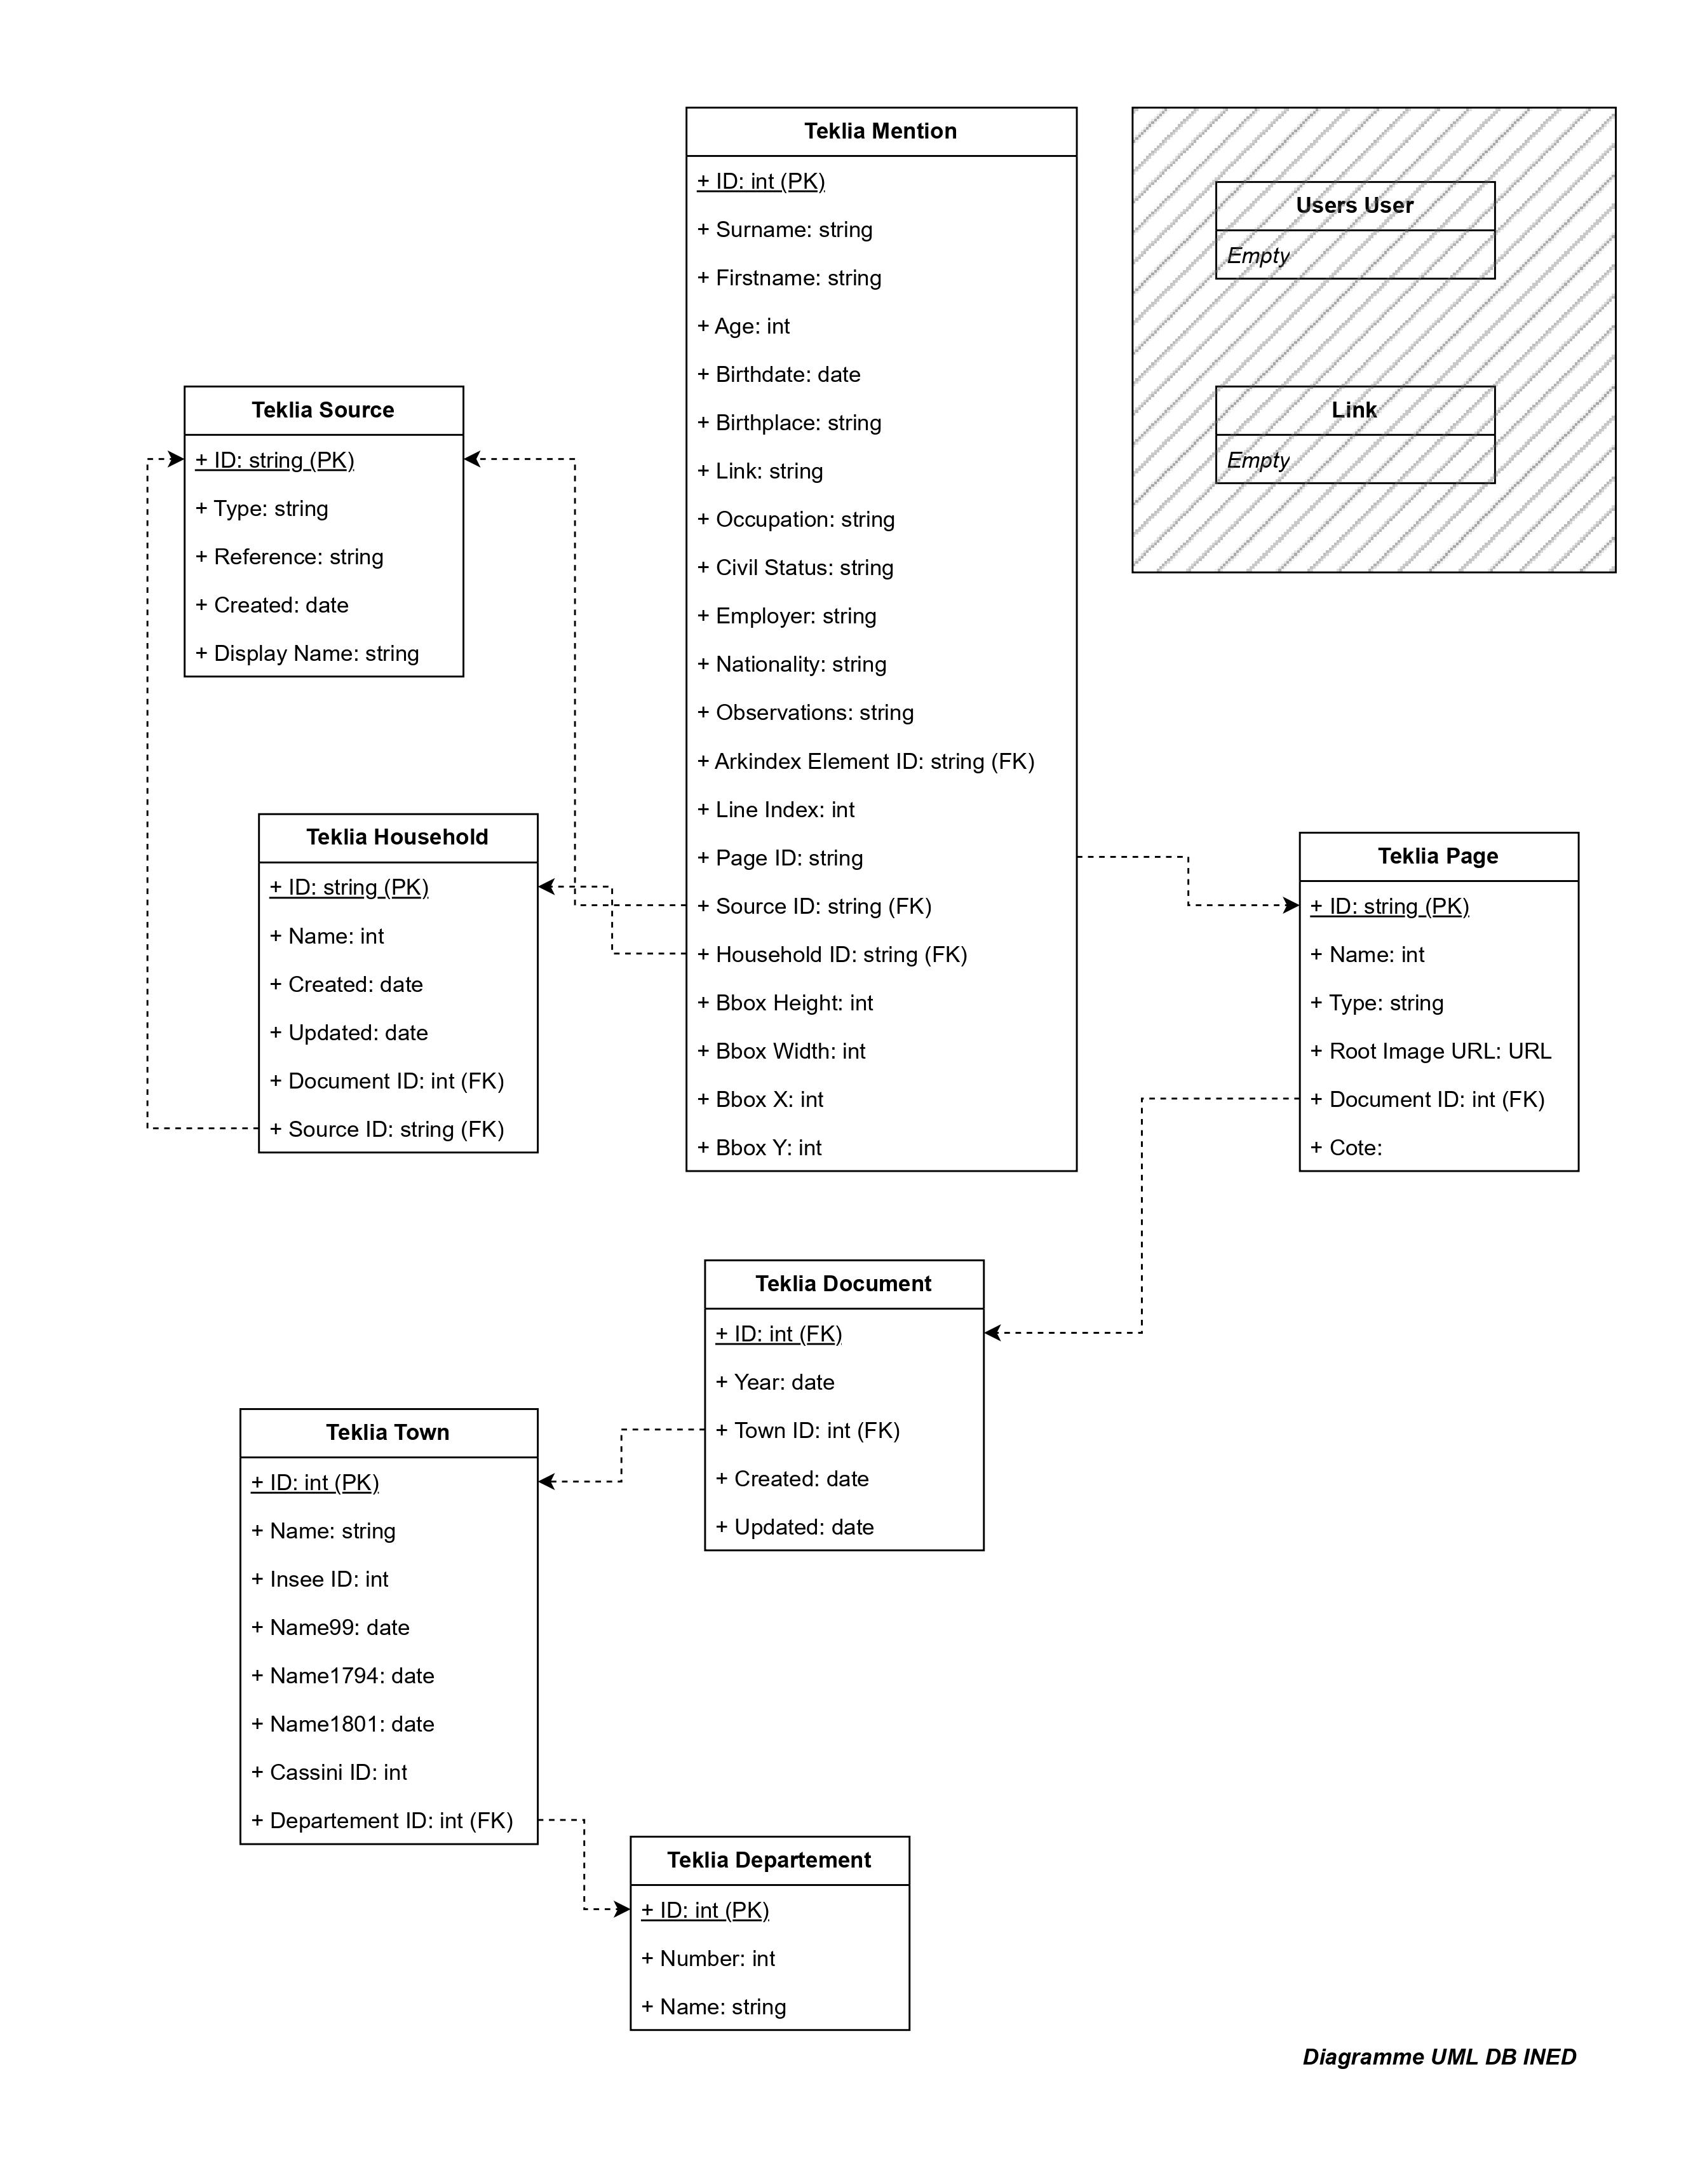
\includegraphics[width=1.0\linewidth]{Figures/Partie 2/Fig.2.1 - Modèle de données - DB INED.jpg}
        \caption[Modèle de données pour la Base de Données]{Modèle de données pour la Base de Données}
        \label{fig:Fig2.1}
    \end{figure}
\clearpage

Plusieurs problèmes vont se poser aux équipes : 
\begin{itemize}[label=\textbullet]
    \item Teklia doit avoir accès à la base de données hébergées sur l’INED pour récupérer les données
    \item Teklia doit pouvoir reverser les métadonnées (collectées par l’outil \\Spider{}{}) dans la base de données de l’INED
    \item FranceArchives (site internet des Archives Nationales) hébergera la base nationale et doit avoir un format pivot interopérable pour reverser les données aux archives départementales et municipales. Pour cela, le SIAF fait appel à un prestataire externe, Logilab.
\end{itemize}

Quelles solutions pour ces problèmes ? 
\begin{enumerate}[label=\alph*)]
    \item \textbf{Concernant le problème de compatibilité entre la base de données de l’INED et celle de Teklia :} 
Pendant un certain temps, les équipes ont réfléchi à la gestion de deux bases de données distinctes : une base de données "\textbf{primaire}" (ou \textit{Master}) et une base de données "\textbf{répliquée}" (ou \textit{slave}). Étant donné que le processus de production est géré par \Arkindex{}, un outil de Teklia, on aurait pu créer la base de données initiale chez Teklia puis la répliquer sur l'INED pour y effectuer les modifications. Ce n'est pas la solution choisie, même si elle aurait tout aussi simple. Mais Teklia verse les données, tandis que l'Ined les travaille et les modifie, il était donc plus logique de procéder ainsi.  
Il y a aussi la solution multimaster, c’est-à-dire dans laquelle les deux bases auraient été considérées comme "\textbf{primary}" et où les écritures peuvent être faites sur les deux avec une synchronisation. Mais cette solution a également été écartée car elle nécessite un logiciel propriétaire et n’est pas très stable, d’autant plus qu’on parle de bases de données d’un poids considérable. 
Il a donc été décidé que la base de données "\textbf{primary}" serait hébergée par l’INED et la "\textbf{replica}" chez Teklia. Un dernier obstacle existait : trouver un système de gestion de base de données compatible sur les deux serveurs. Le choix s’est porté sur PostgresSQL, un modèle répandu et utile pour les bases de données relationnelles. Par ailleurs, les techniciens informatiques de l’INED ont accepté d’ouvrir leurs serveurs à Teklia pour permettre à leurs équipes de travailler dessus et de pouvoir connecter les deux bases pour reverser des données. 
    \item \textbf{Concernant France Archives :}
Dans un premier temps, le SIAF a décidé de travailler à partir d’un "\textbf{dump}". Un "\textbf{dump}" est une sauvegarde d’une base de données (contenu et structure) à un moment donné. La différence avec la réplication c’est que la base n’est pas connectée à la base "\textbf{primaire}", il n’y a donc pas de synchronisation régulière. Mais cela permet au SIAF de commencer à travailler sur la structure de la base, même si les données en elles-mêmes sont amenées à évoluer à mesure que le projet avancera. Par ailleurs c’est une technique beaucoup plus stable, puisqu’il n’y a pas de mises à jour régulières. A terme, le SIAF utilisera un serveur dédié afin d’héberger une réplication de la base de données, afin de la rendre accessible sur leur site internet. 
Ces problèmes techniques découlent de deux éléments: l’ampleur des données traitées, qui nécessite une typologie particulière de serveur et de système de gestion de base de données, et le nombre d’acteurs impliqués, du fait que le projet est interdisciplinaire. Mais en réalité, ces éléments sont liés : l’ampleur des données nécessite une collaboration entre des acteurs aux expertises diverses. Cette collaboration nécessite un travail important sur l’articulation des moyens techniques. Et cette articulation est rendue plus difficile par l’ampleur des données. Un projet monodisciplinaire n’aurait pas connu ces difficultés, car il n'y aurait pas eu d’efforts à faire pour trouver un moyen de partager la base de données à tous les acteurs (dans le cas où il n’y aurait pas de collaboration entre différentes institutions). Ici c’est la collaboration entre plusieurs types de personnes qui pose problème : si le projet n’avait été porté que par l’INED, la base de données serait restée sur leur serveur, et ils auraient pu la gérer comme ils l’entendent, y ajouter des données ou en retirer. Mais ce serait supposer que l’INED possède la technologie suffisante et l’expertise nécessaire pour construire un tel outil. Ce n’est pas le cas et c’est pourquoi ce projet est en collaboration et interdisciplinaire.\\

En résumé, la gestion des données au sein du projet SocFace met en évidence les défis techniques et organisationnels posés par l'ampleur des informations traitées et la diversité des acteurs impliqués. Le caractère interdisciplinaire du projet, essentiel pour exploiter pleinement les compétences de chaque partenaire, complexifie l'articulation des moyens techniques nécessaires. De même, la collaboration entre institutions, bien que cruciale pour le succès du projet, entraîne des difficultés supplémentaires, notamment en ce qui concerne le partage et la synchronisation des données. Il est donc fondamental de développer des solutions adaptées pour assurer la cohérence et l'efficacité de l'ensemble du processus. C’est pour cela que les porteurs du projet ont cherché utiliser un outil de visualisation des données, pour offrir une synthèse claire et accessible des informations collectées à tous les acteurs du projet. Ce type d'outil permet non seulement de suivre l'évolution du projet, mais aussi de fournir aux partenaires, notamment les services d'archives, une représentation visuelle des données traitées.
\end{enumerate}



 \chapter{Gérer un outil de visualisations de données}

Comme on l’a vu, manipuler la base de données issue du processus de production n’est pas particulièrement aisé. Cela requiert des moyens importants, et une expertise technologique poussée. Or il faut pouvoir donner la possibilité de visualiser les données à certains partenaires du projet, notamment les services d’archives qui n’ont pas ces moyens ou cette expertise. C’est pourquoi il a été décidé de recourir à un outil d’analyse et de visualisation de données, plus simple à manipuler. 

\section{Une base de données, pour qui?}

L’un des objectifs du projet SocFace est de permettre aux services des archives départementaux et municipaux de valoriser leurs fonds documentaires. Comme mentionné précédemment, les listes de recensements sont des ouvrages volumineux et difficiles à manipuler, ce qui incite ces services à s'engager dans le projet. Cependant, les archives ne pourront pas accéder à la base de données finale avant la fin du projet, en 2025. Dans l'intervalle, il est donc essentiel de leur fournir des informations exploitables sur les images qu’ils ont contribué à numériser.\\
SocFace a donc cherché à mettre en place un outil de visualisation des données, qui, bien que limité, permet de donner un aperçu des volumes traités. Contrairement à un système de gestion de base de données classique, cet outil n’a pas pour vocation de faciliter la recherche approfondie, comme la consultation de noms spécifiques ou de communes. Il s'agit plutôt de générer des visualisations synthétiques, telles que des graphiques, des histogrammes ou des diagrammes en camembert, afin de donner une vue d'ensemble des données traitées. Ce type d’analyse légère permet aux services d'archives de suivre l'état d'avancement du projet, en attendant la mise à disposition de la base de données complète, qui sera développée en collaboration avec le SIAF. En parallèle, cet outil sert également les besoins internes du projet SocFace. Lancé il y a deux ans, il est crucial de réaliser des points d’étape réguliers pour évaluer l’avancement et ajuster les efforts si nécessaire. De plus, ces visualisations sont précieuses pour les présentations lors de conférences ou autres événements de valorisation de la recherche, offrant ainsi une meilleure visibilité sur les progrès accomplis. Dans les deux cas, l’objectif est de créer un tableau de bord personnalisé pour chaque département, permettant de suivre l'évolution de la production de leurs données, notamment les mentions (noms, professions, âges, etc.) et les métadonnées (communes, dates, départements). Idéalement, ce tableau de bord sera dynamique et connecté à la base de données de l’INED, offrant ainsi une mise à jour en temps réel de l’état des travaux.

\section{Metabase, un bon choix?}
Afin de réaliser ce tableau de bord, les équipes de SocFace ont choisi la solution offerte par Metabase . C’est un outil de Business Intelligence (\textit{ensemble des outils, des technologies et des méthodes utilisés pour collecter, analyser et présenter des données d'une entreprise. L'objectif est d'aider les décideurs à mieux comprendre les performances de l'entreprise et à prendre des décisions éclairées. En d'autres termes, la BI transforme des données brutes en informations utiles pour guider les stratégies et les actions d'une entreprise}). C’est un outil en open source, ce qui signifie que son code est ouvert et son utilisation autorisée pour tous (sous réserve de respecter la licence sous laquelle le programme est distribué).\\
Metabase fonctionne par connexion à une base de données. C’est très utile pour les bases de données de grande ampleur comme c’est le cas pour SocFace, puisqu’il n’y a pas de téléchargement de la base de données et donc pas de limite au nombre de lignes possibles. Un autre avantage est que les données sont mises à jour automatiquement. Mais cela implique aussi des contraintes techniques, puisqu’il faut avoir un accès au serveur et celui-ci doit être stable.\\
En termes de fonctionnement, Metabase est très intuitif : basé sur les requêtes SQL\footnote{Voir Glossaire}, il permet à des novices, qui ne possèdent pas ce langage, de pouvoir interroger la base de données. Grâce à une interface très simple, l’utilisateur est invité à exprimer son besoin, et le programme transforme sa question en requête SQL, de façon transparente. On peut également indiquer sa propre requête SQL si on maîtrise le langage, pour effectuer des requêtes plus complexes. Une fois les données agrégées en réponse à notre question, on choisit le type de visualisation qui nous convient. Les différentes visualisations sont associées pour créer un tableau de bord. 

\begin{figure}[H]
        \centering
        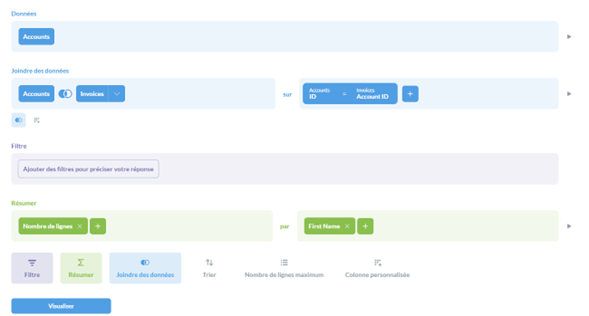
\includegraphics[width=1.0\linewidth]{Figures/Partie 2/Fig.2.2 - Metabase.png}
        \caption[Interface Metabase - Formuler une question]{Interface Metabase - Formuler une question}
        \label{fig:Fig2.2}
    \end{figure}

Concernant le projet SocFace, nous nous en sommes servis pour créer des tableaux de bord pour les premiers départements à avoir intégré la base de données. Les tableaux de bords reprennent uniquement les métadonnées c’est-à-dire les informations sur ce qui est entré dans la base de données, mais pas sur les données elles-mêmes. 
\clearpage

\begin{figure}[H]
        \centering
        \includegraphics[width=0.95\linewidth]{Figures/Partie 2/Fig.2.3 - Metabase - Visualisation pour le Puy-de-Dôme.jpg}
        \caption[ Metabase - Visualisation pour le Puy-de-Dôme]{ Metabase - Visualisation pour le Puy-de-Dôme}
        \label{fig:Fig2.3}
    \end{figure}

Sur cet exemple, nous pouvons ainsi voir : 
\begin{itemize}
    \item Un tableau croisé dynamique sur le nombre de pages traitées, par année et par commune ;
    \item Un tableau croisé dynamique sur le nombre de pages traitées, par année et par commune ;
    \item Le nombre de commune dans le département ;
    \item Le nombre de pages total traité et par année sur un camembert ; 
    \item Le nombre de document traité par année, qui correspond à peu près au nombre de commune puisqu’il y a un document par commune ; 
    \item Le nombre de page traité par année sur un histogramme ;
    \item La comparaison entre le nombre de pages traitées pour le Puy-de-Dôme et les autres départements traités. 
\end{itemize}

Une fois ces tableaux élaborés, l’idée était de les automatiser afin de pouvoir créer ces tableaux pour chacun des départements et qu’ils soient mis à jour en synchronicité. Malheureusement, Metabase ne permet pas cette automatisation. S’il y a une mise à jour sur la base de données, il faut repasser par la procédure de question. Cela nécessiterait donc que chaque service d’archive utilise directement Metabase et crée son propre tableau de bord. Là encore, ce n’est pas possible car Metabase est connecté à un serveur de l’INED qui héberge la base de données. Or on ne peut pas se connecter à ce serveur hors de l’établissement de l’INED au Campus Condorcet, pour des raisons de sécurité. Par ailleurs, le traitement par le programme des questions peut être très long. Lorsque nous avons créé les tableaux de bord « tests », il n’y avait que 24 départements et le temps de chargement des résultats pouvait parfois prendre plus de 3mn. En supposant que les 98 services d’archives qui ont donné leur accord envoient bien leurs images, il va être très difficile d’obtenir de bonnes performances via Metabase. \\

Cet outil était donc adéquat pour les besoins du projet : permettre à des novices en langage \gls{SQL} de pouvoir élaborer des tableaux de bords de suivi du projet. C’était intéressant dans un contexte d’interdisciplinarité car tous les membres du projet ne sont pas compétents en SQL. Dans l’hypothèse où on aurait laissé les services d’archives accéder à l’outil, ils auraient pu générer leurs propres visualisations sans trop de complexité. \\
Il ne sera donc pas retenu pour cette utilisation, mais reste un outil intéressant pour une utilisation interne au projet, et peut servir de supports pour une valorisation du projet lui-même. Il faut simplement admettre qu’il ne pourra pas être automatisé et demandera donc une certaine maîtrise de l’outil par l’utilisateur. 





 \chapter{La question de la fiabilité des données}

On a donc vu que la donnée empruntait un chemin ardu, à travers plusieurs outils et sous plusieurs formes. Différentes équipes travaillent à différents moments sur ces données. Ces équipes ont des niveaux différents d’expertises de la donnée. Il est donc primordial de s’assurer de la fiabilité de ces données. Ainsi, il faut évaluer les performances des outils \Spider{} et \Arkindex{}, qui sont les principaux outils permettant à la donnée d’intégrer une base. Se pose également la question des serveurs, qui sont essentiels au projet, puisque l’ampleur des données collectées nécessite un endroit de stockage important, stable et accessible aux différentes équipes. On verra que conserver 100\% de l’intégralité des données est difficile dans un projet aussi complexe, aussi, il est intéressant d’anticiper la perte des données. 

    \section{Les performances des outils du projet, \Spider{} et \Arkindex{}}

Pour rappel, \Spider{} est l’outil qui permet d’associer les images numérisées par les services d’archives avec leurs métadonnées avant d’intégrer \Arkindex{}, la technologie HTR développée par Teklia. \Spider{} fait des erreurs, et il faut parfois relancer le processus plusieurs fois pour s’assurer que toutes les images sont traitées. Mais l’avantage est que l’outil prévient du nombre d’erreur. Dans ce cas, il faut explorer le fichier de métadonnées fourni par les services d’archives pour comprendre ce qui ne fonctionne pas. Cela ne requiert pas d’expertise particulière mais c’est réalisé par les équipes d’ingénieurs chez Teklia. 
C’est surtout lors du travail d’\Arkindex{} que la question de la fiabilité des données va se poser. Il faut cependant distinguer deux types de données. De fait, \Arkindex{} "double" la donnée : 

\begin{samepage}
\begin{itemize}
    \item On a toujours la donnée contenue dans les images numérisées
    \item On récupère la donnée créée à partir de ces images par le processus HTR
\end{itemize}
\end{samepage}
Il faut s’assurer de l’intégrité et donc de la fiabilité de ces deux types de données.\\

Concernant les images numérisées, c’est-à-dire les mots contenus dans les livres de recensement, on ne peut que faire confiance à ceux qui les ont rédigés, et accepter cette réalité telle quelle. Cependant, il y a un point à explorer : ces livres de recensement ont été aussi utilisés par les annotateurs pour nourrir et entraîner les modèles, comme \DAN{} ou \YOLO{} qui travailleront sur les images pour lire, reconnaître et extraire les données. Les annotateurs vont donc indexer, à la main, des listes de recensement : ils font le travail – manuellement – que les modèles seront amenés à faire par la suite de façon automatisée.  Les équipes d’annotateurs commencent par définir des zones\footnote{Extraits du mode d'emploi destiné aux annotateurs.} : 

\clearpage
\begin{figure}[H]
        \centering
        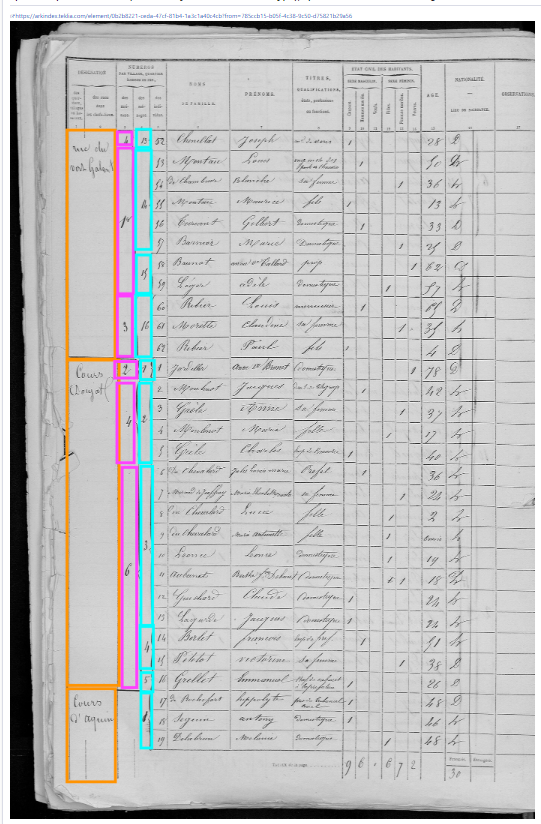
\includegraphics[width=0.8\linewidth]{Figures/Partie 2/Fig.2.4 - Exemple d'une page avec délimitation des zones - Mode d'emploi SocFace à destination des annotateurs.png}
        \caption[Exemple d'une page avec délimitation des zones]{Exemple d'une page avec délimitation des zones}
        \label{fig:Fig2.4}
    \end{figure}

Ceci n’est qu’un exemple, car les listes de recensement ont évolué dans leur format au fil du temps. C’est pourquoi il est primordial d’entraîner les modèles sur les différents types de listes que l’on peut trouver.\\ 
\clearpage
La deuxième étape, c’est l’indexation des mentions. On le voit, l’écriture n’est pas toujours simple à déchiffrer et dans certains cas, le scripteur a utilisé une abréviation. 
\begin{figure}[H]
        \centering
        \includegraphics[width=0.95\linewidth]{Figures/Partie 2/Fig.2.5 - Exemple des champs à remplir pour l'annotation.png}
        \caption{Exemple des champs à remplir pour l'annotation}
        \label{fig:Fig2.5}
    \end{figure}

Ainsi, une partie du traitement est manuelle, et un humain est plus susceptible de faire une erreur qu’une machine, même si on verra que les machines en font aussi. En effet, lorsque les modèles travaillent sur la lecture des données, on voit qu’elles peuvent avoir ce qu’on appelle des hallucinations : cette technologie est prédictive, elle utilise les informations qu’on lui a fourni pour prédire à son tour la nature des mentions qu’elle lit. Mais ces technologies basées sur le \gls{DL} ne peuvent pas admettre quand elles ne savent pas ou quand elles doutent. Dès lors, elles vont « reconnaître » un mot ou une date qui n’est pas la bonne. On dit qu’elles ont des hallucinations. Ou bien ne pas voir qu’il s’agit de deux pages différentes ou qu'une page se termine. Cela peut s’expliquer par une mauvaise numérisation, avec un contraste faible, ou bien une mauvaise qualité de la source elle-même (bien que les listes de recensement soient dans l’ensemble bien conservées). Il peut également avoir des problèmes au moment de l’export \Arkindex{} vers Teklia. L’HTR se comporte correctement mais au moment de l’export, des lignes sont manquantes ou des mentions n’existent plus.\\
SocFace est un projet complexe et multidisciplinaire. Le type d’erreur découle de la technologie utilisée, mais également du fait que le chemin de la donnée emprunte différent support. La base de données finale est le résultat conjoint de la technologie, mise au point par des ingénieurs informatiques de Teklia, des annotations faites par des annotateurs recrutés et l’analyse des chercheurs de l’INED. C’est le fruit d’une interdisciplinarité et d’une collaboration entre différents acteurs. C’est une nécessité pour le projet, mais c’est également l’une des raisons pour lesquelles ces erreurs peuvent arriver. La donnée est produite par la conjonction de plusieurs expertises, mais au prix d’un processus long et dont les étapes sont opérées par des acteurs différents. Encore une fois, on voit que l’interdisciplinarité est nécessaire, mais également à l’origine de questionnements sur le projet, en l’espèce sur la fiabilité même des données. 

    \section{Plusieurs serveurs pour une donnée fiable}

La question des serveurs est bien évidemment primordiale pour gérer la pérennité des données.  Ces serveurs jouent deux rôles :
\begin{itemize}[label=\textbullet]
    \item Ils apportent \textbf{la puissance de calcul} pour le processus de lecture et d’extraction des données
    \item Ils permettent \textbf{le stockage des données}, que ce soit les images numérisées, puis la base de données elle-même.
\end{itemize}

Concernant la puissance de calcul, elle est nécessaire pour mener à bien le processus. En l’espèce, vu le nombre considérable de pages à traiter et de données à extraire, il est nécessaire de s’appuyer sur un supercalculateur. SocFace utilise donc Jean Zay, qui appartient et est maintenu par le CNRS. Pour avoir le droit d'utiliser ce serveur, qui est un des plus puissants d'Europe\footnote{\href{https://www.top500.org/lists/top500/list/2024/06/?page=4}{https://www.top500.org/lists/top500/list/2024/06/?page=4}}, il faut démontrer un projet de recherche, non commercial, et d'une expertise suffisante des membres de l'équipe. Ici, SocFace a demandé 200 000 heures d'utilisation.
Cette puissance de calcul est d’autant plus nécessaire pour SocFace que comme on l’a vu, \Arkindex{} effectue l’ensemble des opérations de reconnaissance du texte manuscrit en un seul passage, contrairement à ce qui se fait en principe dans ce genre de projet. C’est un modèle intégré. Or, plus le serveur est puissant, plus les résultats sont solides : cela limite le nombre d’erreurs, ou d’hallucinations possibles. Il fallait donc pour SocFace un supercalculateur. Si Jean Zay est nécessaire, il est aussi instable. Le projet est tributaire de la maintenance par le CNRS, des mises à jour, et des nombreuses autres utilisations qui sont faites du supercalculateur. Cette collaboration est nécessaire, mais est à l’origine de certains ralentissements et nécessite aux équipes du projet de s’adapter.\\
Concernant les serveurs pour le stockage des données, ils sont plus nombreux. Comme on l’a vu, Teklia a ses propres serveurs, et ils sont utilisés pour stocker les images numérisées avant l’intégration des données, puis lors du traitement sur \Arkindex{}. Mais par la suite, la base de données est hébergée par un serveur de l’INED. Elle est répliquée sur un serveur de Teklia, et à terme, le SIAF aura également sa propre base de données sur ses propres serveurs. Cela fait donc trois serveurs pour trois bases de données, qui ne doivent pas être dissociées, car il faut s’assurer de l’adéquation des bases de données entre elles. A ce jour, la base de données du SIAF n’existe pas (comme on l’a vu, ils travaillent pour l’instant sur un dump), on ne peut donc pas présager d’une dissociation ou d’une perte des données. Concernant Teklia et l’INED, c’est une réplication, avec une synchronisation en temps réel, pour empêcher ce genre de problèmes. Cette connexion peut poser des problèmes. En effet l’INED est une institution publique. 
\\A ce titre, il y a certaines contraintes : 

\begin{itemize}
    \item Respect des protocoles de sécurité, pour protéger le réseau
    \item On ne peut pas permettre l’accès au serveur à n’importe qui, il faut donc privilégier les ingénieurs qui travailleront dessus
    \item Le serveur de l’INED est partagé avec tous les autres équipes de recherches de l’INED, SocFace ne peut donc pas agir à sa guise et doit passer par les équipes IT de l’INED.
\end{itemize}

Par exemple, utiliser Metabase ailleurs qu’à l’INED s’est révélé impossible car le programme est connecté au serveur de l’INED. Jongler entre ces différents serveurs nécessite une bonne communication entre les équipes qui collaborent. Il faut s’adapter constamment pour trouver des solutions, là où dans un projet mené par un seul acteur ou dans une seule discipline, la question se serait moins posée car ils auraient pu disposer de leur propre serveur. Et dans le même temps, ce type de projet n’aurait sûrement pas eu la même envergure et n’aurait pas eu besoin d’autant de puissance et de stockage. \\
On voit donc que les outils et les serveurs utilisés pour le projet, s’ils sont nécessaires et pensés pour traiter des données de grande ampleur, ne sont pas à l’abri de provoquer des erreurs dans l’écriture des données. Comment dès lors anticiper ce qui peut amener à une perte des données ou à leur dégradation ?


    \section{Comment palier la perte des données?}

Les équipes de SocFace doivent composer avec la possibilité d’erreurs dans les données, que ce soit dans l’indexation, dans le transfert ou dans l’écriture de la donnée. Comment anticiper cela ? Quel seuil d’erreur est acceptable ? Comment régler les erreurs une fois qu’elles sont repérées.\\ 

On l’a vu, les erreurs peuvent intervenir dès l’entraînement des modèles par les annotateurs qui utilisent le système Callico. Pour limiter au maximum les erreurs humaines, SocFace a produit de la documentation avec des consignes à suivre\footnote{Voir Annexe G} . Cela permet également d’assurer une certaine cohérence dans les données. Par exemple, conserver les accents, développer les abréviations, corriger les fautes d’orthographe évidentes etc… Il faut aussi comprendre que les difficultés ne sont pas les mêmes selon le type de mention : il est plus facile de se tromper sur un nom de famille peu courant que sur une année où les combinaisons différentes sont beaucoup moins nombreuses que pour un mot. Cela permet également de normaliser les mentions. Par exemple, s’assurer que la mention "cultivateur", souvent abrégée en "culti", soit bien développée. 
Pour autant, malgré l’encadrement des annotateurs, il peut y avoir des erreurs. C’est le cas pour la mention "idem" ou "id.". Cette mention est très utilisée par le scripteur, pour simplifier son travail. On la trouve notamment dans la colonne « nationalité » ou pour le nom de famille d’un même foyer. Certains annotateurs ont développé le "idem" en réécrivant la mention. Il a donc fallu développer un programme pour récupérer la mention "idem" à la place de la réécriture de l’annotateur. Ce type de correction manuelle sont faites à posteriori, une fois que les erreurs ont été détectées. On peut l’utiliser pour d’autres types d’erreurs qui ont été repérées ou pour favoriser la normalisation. Par exemple retirer le "ans" lorsque l’âge est mentionné.\\
Ces erreurs sont donc détectées après l’écriture des données dans une procédure de "nettoyage". Les chercheurs de l’INED qui ont accès à la base de données navigue à travers les données déjà produites afin de voir les incohérences qui peuvent ressortir. Au vu de l’ampleur des données, il est bien entendu impossible de faire une vérification précise. Par exemple, une des expériences tentée a été de comparer le nombre de mention de nom par commune – c’est-à-dire le nombre d’habitant – avec les chiffres de l’INSEE sur les mêmes années. Si les chiffres divergent trop, cela signifie certainement qu’il manque des pages sur la commune ou bien qu’il y a eu un doublement de l’export des données. Ces tests sont effectués majoritairement par les chercheurs de l’INED. Dans tous les cas, il faut avoir un accès à la base de données pour cela, et ce n’est pas le cas de tous les membres de l’équipe. Mais cela reste un bon exemple de collaboration interdisciplinaire : un développeur peut créer un script de correction de données en se basant sur les analyses faites par un démographe.\\

On voit donc que des moyens sont mis en place pour limiter les possibilités d’erreurs. Soit par anticipation, soit par correction, une fois les erreurs détectées. Mais dans les deux cas, il faut accepter un taux d’erreur possible. On parle de la numérisation de près de 15 millions de pages et donc l’écriture de plusieurs centaines de millions de mentions. Il faut donc déterminer un seuil d’erreur acceptable, qui devra être pris en compte par les chercheurs dans leur réutilisation de la donnée.

Ce chapitre a permis de souligner l’importance de la gestion des données dans le projet SocFace. La nature complexe et diversifiée des données, ainsi que les multiples acteurs impliqués imposent des défis techniques et juridiques significatifs. En détaillant les processus de collecte, d’intégration, de visualisation et de sécurisation des données, nous avons montré comment ces éléments se conjuguent pour transformer des informations brutes en une base de connaissances structurée, apte à soutenir des recherches futures. L’interdisciplinarité, au cœur du projet, exige une collaboration étroite et une harmonisation continue des efforts pour maintenir l’intégrité et la cohérence des données, tout en respectant les cadres légaux en vigueur. Après avoir vu ces considérations techniques et organisationnelles, nous allons explorer plus en détail les perspectives offertes par l’analyse de ces données : les méthodologies employées pour extraire des connaissances pertinentes des vastes ensembles de données accumulées, ainsi que les enjeux liés à l’exploitation de ces données dans un cadre de recherche. 
	
    \part{Les perspectives offertes par l’interdisciplinarité : SocFace au cœur de la Recherche}

Collaboration et interdisciplinarité irriguent le projet. Rendues nécessaires par l’ambition des objectifs de SocFace, cela oblige des équipes a priori très différentes à travailler ensemble Face à l’ampleur croissante des données, la collaboration entre entreprises privées et institutions de recherche s'avère incontournable. Nous examinerons d'abord comment ces deux mondes peuvent unir leurs forces. Ensuite, nous analyserons la contribution de ces collaborations à l’évolution de la recherche et enfin, nous explorerons les perspectives futures, en mettant l’accent sur les défis techniques à venir et les nouvelles applications possibles.
\vspace*{\fill}
\begin{center}
  % Ajouter un joli cadre autour de l'image
  \setlength{\fboxsep}{5pt}  % Espace entre l'image et le cadre
  \setlength{\fboxrule}{1pt} % Épaisseur du cadre
  \fbox{
    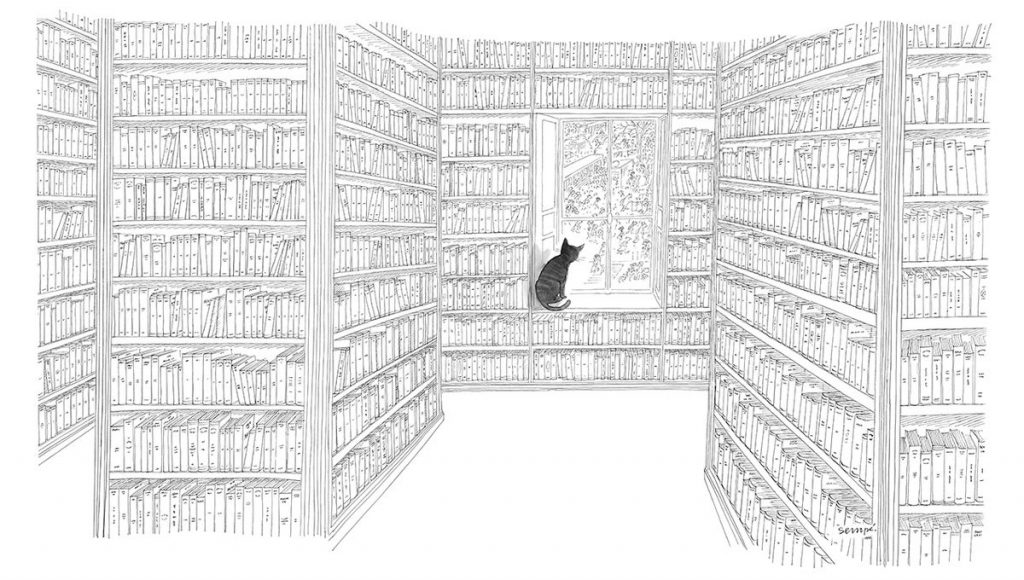
\includegraphics[width=0.8\textwidth]{Figures/Partie 3/Illus.Partie 3.png}}\\
    \vspace{0.5em} % Espace entre l'image et la légende
    {\scriptsize \textit{Crédit : Sempé.}}
\end{center}

\chapter{Le meilleur des deux mondes pour affronter des données d’ampleur}

Les objectifs ambitieux de ce projet nécessitent une collaboration étroite entre des acteurs aux compétences complémentaires, combinant la technologie avancée des entreprises avec la rigueur scientifique des institutions publiques. Cette collaboration ne se limite pas à une simple nécessité pratique mais s’inscrit dans un contexte historique et socio-économique où les collaboration entre public et privé sont devenus une réponse à la diminution des financements publics. Dans ce cadre, SocFace illustre les bénéfices de cette coopération pour mener à bien des projets d’envergure. Nous examinerons d’abord comment cette alliance s’est développée, avant d’analyser les avantages pour les entreprises privées, puis de discuter des limites des institutions publiques dans ce type de collaboration. 

    \section{La nécessité des uns pour les autres, travailler ensemble}

La littérature centrée sur la recherche partenariale commencent toujours par nous rappeler le contexte dans lequel se sont développés ces partenariats. Jusque dans les années 80, la recherche publique restait le plus souvent initiée, opérée et financée par des agents publics. Cette politique est le fruit d’une longue institutionnalisation des centres de recherches et universités françaises. Mais avec le développement de la mondialisation, le mouvement de privatisation que connaît une partie des pays développés, le budget alloué à la recherche a baissé. On peut prendre les chiffres avancés par le rapport de la mission sur l’écosystème de la recherche et de l’innovation\footnote{\fullcite{rapport_mission}}. Il avance dans un premier temps que les investissements de l’ANR dans la loi pour la recherche de 2030 sont en augmentation : 

\begin{figure}[H]
        \centering
        \includegraphics[width=1.0\linewidth]{Figures/Partie 3/Fig.3.1 - Schéma ANR.png}
        \caption{Budget d’intervention hors investissements d’avenir/France 2030 et mesures de préservation de l’emploi dans la R\&D privée prévues dans le plan de relance.\\
        \textit{Crédit : ANR}}
        \label{fig:Fig3.1}
    \end{figure}

Cela se traduit par des effets positifs : le taux de réussite des appels à projets de l’ANR en 2022 est de 24\%, alors qu’il ne dépassait pas les 10\% en 2010. Mais ces chiffres ne doivent pas masquer une autre réalité : le budget global alloué à la recherche ne dépasse pas l’objectif de 3\% fixé par les différents gouvernements depuis des décennies. C’est un des plus bas des pays de l’OCDE selon le rapport. Ainsi, les budgets de fonctionnement des laboratoires et centres de recherches sont en baisses constantes. Par exemple, le rapport d’Auto-Evaluation du CNRS décrit ainsi son budget au cours des dix dernières années : 

\begin{quote}
\textit{"Entre 2012 et 2021, le CNRS a perdu 4,3\% de ses effectifs rémunérés sur la subvention pour charges de service public (24 685 contre 25 787) alors que dans le même temps, la part de cette subvention consacrée aux dépenses de personnel est passée de 82,2\% à 84,1\%. Mécaniquement, le pourcentage de la subvention disponible pour le fonctionnement et les investissements a diminué de 2\%, passant de 17,4\% à 15,4\%. Cette « double peine »  moins de personnel et un budget de fonctionnement et d'investissement plus faible  a manifestement réduit la capacité de l'organisme à développer et à mettre en œuvre une véritable politique scientifique".}  
\end{quote}

Avec ce genre de politique, on comprend que la recherche partenariale soient encouragés. On pourrait presque penser que cela permet aux pouvoirs publics de se désengager de la recherche. Pour autant, concernant le projet SocFace, la situation est plus complexe : il n’y a pas eu de financement privé, dans le sens où aucune entreprise n’a fourni d’argent pour le projet. Mais l’un des porteurs principal du projet est une entreprise privée et fourni dès lors sa propre technologie, son expertise, ses locaux et surtout sa main d’œuvre. C'est un apport en nature. Il y a donc un soutien privé, qui pallie le manque de budget de la recherche considéré à plus large échelle. De fait, on peut supposer que si la recherche, depuis tant d’années, avait été mieux financée, la technologie développée par Teklia aurait pu été développée par l’INED directement. Bien entendu, cela reste une supposition, qui ne peut absolument pas être vérifiée.\\ 

SocFace semble toutefois indiquer que le recours à la recherche privée devient une nécessité pour gérer ce type de projet. Reste à trouver l’entreprise qui correspond à ce besoin, qui doit également y trouver son intérêt. 

\section{De l'intérêt d'entrer dans la recherche pour Teklia}

Quel est intérêt de participer à projet de recherche pour Teklia, entreprise spécialisée dans le traitement automatique des documents et des données massives et qui est déjà à la pointe de l’expertise en intelligence artificielle, en vision par ordinateur et en traitement du langage naturel. \\

D’une part, on peut penser que ce partenariat participe du mouvement initié par les pouvoirs publics depuis quelques années en matière d’incitation à la recherche. La politique fiscale tente en effet de favoriser la participation du secteur privé à l’innovation, motivant les start-ups avec des crédits d’impôts. Teklia ayant été créé en 2014, on ne peut plus vraiment la considérer comme une start-up mais elle est désormais une entreprise installée et innovante. Ainsi, on a le Crédit d'Impôt Recherche (CIR) qui permet aux entreprises de bénéficier d’un crédit d’impôt équivalent à 30\% des dépenses de recherche et développement (R\&D) jusqu'à 100 millions d'euros, et 5\% au-delà. Le CIR couvre les dépenses liées aux salaires des chercheurs, à l'achat de matériel, aux frais de sous-traitance de la recherche etc.... Cela réduit considérablement le coût net des projets de recherche pour l’entreprise. Les chiffres les plus récents datent de 2021 et font état d’un montant de 7,25 milliards d’euros de crédit. On doit donc que c’est une incitation qui fonctionne. \\
D’autre part, on a vu dans l’explication du déroulement du projet que la technologie développée par Teklia nécessitait une forte puissance de calcul, puisque l’ensemble des opérations sont faites en une seule passe. C’est pourquoi SocFace utilise Jean Zay, du CNRS. On peut penser que sans sa participation à un projet de recherche publique, Teklia n’aurait pas eu accès à un outil aussi puissant et aussi sophistiqué. Aussi, il est intéressant pour Teklia de tester sa technologie sur un corpus aussi énorme que les listes de recensement. C’est un défi de taille qui ne peut que permettre d’améliorer leurs outils et affiner leur technologie. Il y a donc aussi un intérêt pour leur politique de développement.\\
Enfin, Teklia est une entreprise, qui produit des solutions pour des clients. Le fait de participer à un projet de recherche publique est une très bonne carte de visite auprès de potentiels clients d’institutions publiques. Ce genre de marché est intéressant pour eux puisqu’ils sont spécialisés dans la lecture de manuscrits, généralement possédés par des institutions du patrimoine, généralement publiques. SocFace est un projet innovant, qui peut se décliner sur beaucoup de corpus différents. Cela ouvre des perspectives commerciales importantes pour Teklia.\\

Ainsi, on voit que les bénéfices pour une entreprise privée sont aussi très intéressants, tant financiers que dans leurs perspectives de développement technologique ou commerciale. C’est un échange de bons procédés entre institutions privées et publiques.  

\section{Les limites des institutions publiques en matière d'humanités numériques?}

Le fait que SocFace ait eu besoin de recourir à la sphère privée veut-il dire pour autant que l’intervention de la sphère publique en matière d’humanités numériques est limitée ? La réponse n’est pas évidente mais la question mérite d’être posée.\\

Il faut commencer par préciser que la définition des "humanités numériques" est assez large. On peut reprendre la définition donnée par Marie-Laure Massot et Agnès Tricoche, dans un article exposant leurs conclusions sur l’évolution des humanités numériques à l’ENS entre 2017 et 2018\footnote{\fullcite{massotRenewalDigitalHumanities2021}} : 

\begin{quote}
C'est l'exploitation de l'outil numérique dans le processus intellectuel de production et d'analyse des humanités et des sciences sociales, une alliance ayant pour objectif d’optimiser le potentiel d’exploitation et de valorisation des données scientifiques."
\end{quote}   

C’est une définition large et flexible, qui s’adapte à un objet toujours plus mouvant. Il est donc fort probable que ce soit cette absence de définition et de périmètre clair qui empêche la puissance publique de pouvoir favoriser et structurer efficacement les humanités numériques. Il n’y a pas à proprement parler de département "humanités numériques" dans la plupart des universités ou organismes de recherches. La matière "humanité numérique" est distillée dans toutes les disciplines. On pourrait donc trouver ici une limite : les humanités numériques, si elles sont reconnues dans la recherche, ne sont pas encore considérée comme une discipline à part entière et sont maintenues dans un système hybride et le plus souvent rattachées à une discipline académique. 
	
Toutefois, on doit préciser qu’il existe des infrastructures orientées vers les humanités numériques. Huma-Num a justement été crée pour favoriser l’accès, le partage, l’exploitation et la conservation des données numériques produites par la recherche en sciences sociale. Créée en 2013, elle est placée sous la tutelle du CNRS et possède des antennes en région, avec les Maisons des Sciences Humaines. Son objectif est de pouvoir faciliter l’accès aux outils numériques pour des laboratoires, projets de recherches ou chercheurs : stockage des données, gestion des formats, création de bases de données etc… Huma-Num favorise également les discussions européennes et encourage les projets transeuropéens. Pour autant, la structure ne bénéficie pas d’un gros budget : 80 000€ en 2019 et seulement 27 salariés (permanents et non permanents). Cette structure permet davantage d’aider un projet que de lui fournir une véritable technologie. Il permet de créer des consortiums, de faire se rencontrer des équipes pouvant collaborer. On peut penser que c’est pour cela que SocFace n’a pas sollicité l’aide d’Huma-Num. L’ampleur du projet n’était pas compatible avec les capacités d’Huma-Num. Il existe par ailleurs des laboratoires spécialisés en \gls{océrisation}\footnote{Voir Glossaire} et en \gls{HTR}, notamment le LITIS, qui dépend de l’Université de Rouen, et qui mène des recherches poussées en intelligence artificielle. Mais ils sont peu en France et développent leurs propres projets. Ainsi, le LITIS est porteur du projet POPP que l’on a mentionné plus haut.\\
	
On ne peut donc pas dire que les humanités numériques en France ne sont pas aidées, ou invisibles à la recherche. Mais elles ne le sont sans doute pas assez pour permettre un développement à 100\% public de tous les projets. D’où la structuration de SocFace, avec une partie issue de la recherche privée. 




\chapter{L'interdisciplinarité au coeur de l'avenir de la recherche}

L'originalité de SocFace ne réside pas dans son interdisciplinarité. La majorité des projets aidés par l’ANR font intervenir plusieurs disciplines, à divers degrés. De même, la recherche partenariale est de plus en plus valorisés, comme en témoigne la dernière publication de l'ANR\footnote{\fullcite{anr2022}}, qui accorde une attention particulière à ces partenariats. Tout cela démontre que, loin d’être singulier, SocFace s’inscrit dans le mouvement de la science ouverte, qui irrigue le monde de la recherche depuis quelques décennies. Nous examinerons d'abord les éléments du projet qui le démontrent, avant d'en analyser les implications, notamment en ce qui concerne la définition du métier de chercheur.

    \section{S'inscrire dans le mouvement de la science ouverte}

Depuis l’antiquité, la communauté scientifique cherche à partager son savoir avec l’humanité. De même, les scientifiques se sont toujours inspirés les uns les autres, dans un dialogue constant qui a permis les plus grandes découvertes. Le travail scientifique est – depuis toujours – basé sur le partage des découvertes et les grandes avancées sont issues de collaboration, de dialogues entre scientifiques, philosophes, mathématiciens etc… Le mouvement de la science ouverte, tel qu’on l’entend aujourd’hui, est le produit des avancées technologiques récentes qui permettent un accès plus simple et plus immédiat aux découvertes scientifiques. Ce mouvement a donc été théorisé : 

\begin{figure}[H]
        \centering
        \includegraphics[width=1.0\linewidth]{Figures/Partie 3/Fig.3.2 - Schéma Science ouverte.png}
        \caption{Composantes de la science ouverte.\\
        \textit{Crédit : Université de Montpellier}}
        \label{fig:Fig3.2}
    \end{figure}

On retrouve six principes clefs : 

\begin{enumerate}
    \item \textbf{L’accès ouvert} : rendre disponibles les résultats de recherches de façon libre et accessible
    \item \textbf{Les données ouvertes} : rendre les données disponibles, réutilisables et accompagnées de leurs métadonnées pour faciliter leur reproduction. On parle du principe FAIR, Findable (= trouvable), Accessible, Interoperable, Reusable (=réutilisable)
    \item \textbf{Logiciels et codes ouverts} :  on parle ici des codes sources développés dans le cadre du projet de recherche, pour mieux comprendre la méthodologie de la recherche
    \item \textbf{Evaluation ouverte par les pairs} : cela permet d’assurer la transparence des modes d’évaluations et permettre à la communauté scientifique de participer à l’évaluation des travaux de leurs collègues
    \item \textbf{Carnets de recherches ouverts} : on parle des journaux de recherches, afin de mieux saisir les doutes, questionnements, hypothèses que l’équipe de recherche a développé tout au long du projet 
    \item \textbf{Science participative} : faire participer le grand public à des projets de recherche
\end{enumerate}

Depuis vingt ans, la science ouverte est au cœur des préoccupations des organismes de recherche. On favorise l’accès libre aux publications (Cairn, HAL), on pousse les chercheurs à collaborer, on favorise le dialogue entre discipline etc… Nous n’allons pas ici exposer les avantages et les inconvénients de la science ouverte car il est désormais acquis que la science ouverte est bénéfique au monde scientifique et à la recherche. La très grande majorité des projets actuels, particulièrement en sciences humaines, s’inscrivent dans ce mouvement. Il resterait à explorer les questions juridiques, et particulièrement du droit d’auteur, qui continuent de poser problème dans un mouvement qui prône un accès totalement libre. Mais ce n’est pas l’objet de notre propos. \\
Comment SocFace adopte cette science ouverte - au delà de l'interdisciplinarité déjà démontrée?  Il faut commencer par l’objectif final du projet : mettre à la disposition du grand public une base de données de grandes ampleur. C’est la définition même de la science ouverte : l’open access pour tous des résultats d’un projet de recherche. Bien évidemment, en l’espèce les données des listes de recensements, c’est-à-dire les noms et les adresses étaient déjà accessibles. Mais le résultat du projet est la construction de la base de données elle-même et c’est ce qui est laissé en libre accès. Concernant la construction du projet, et particulièrement des outils permettant l’HTR, Teklia s’est basé sur un modèle existant déjà, \DAN{}. Celui-ci a été laissé en libre accès par son créateur Denis Coqueret, comme on l’a vu dans la deuxième partie. Par ailleurs, les équipes ont récupérés certaines données du projet Popp, dont l’objectif est sensiblement identique à SocFace mais limité à Paris sur l’entre-deux guerres. C’est donc un dialogue entre deux projets de recherche, exactement ce qui est encouragé par la science ouverte. Enfin, on a expliqué que les modèles étaient entraînés par des annotateurs. Ces équipes d’annotations sont parfois des spécialistes en généalogies, le plus souvent des étudiants rémunérés. Dans tous les cas ces personnes habituées à ce genre de campagne. Mais ils ne sont pas chercheurs ou n’appartiennent pas à la recherche académique. SocFace s’inscrit donc dans la science participative.\\

SocFace est un bon exemple de projet de la science ouverte, ce qui démontre comment le projet est un projet de son temps. Il s’inscrit dans un contexte général d’ouverture de la recherche à d’autres domaines. Ce qui n’est pas surprenant pour un projet qui place la collaboration et l’interdisciplinarité au cœur de son système de fonctionnement. 

    \section{Vers une évolution du statut du chercheur?}

Ce sont les interactions entre chercheurs et techniciens qui sont au cœur de ce projet et qui en font l’architecture. Cette interdisciplinarité n'est pas nouvelle, et Louis Henry l'évoquait déjà dans un article de 1968\footnote{\fullcite{henry}}. Selon lui, les \textit{hommes de l'art} peuvent être des ingénieurs, des chercheurs ou des industriels. Les choses ont-elles évoluées en 50 ans? \\
Pour commencer, on peut dire qu'elle est désormais recherchée et valorisée. Ce dialogue n'est bien évidemment pas apparu avec le numérique, et déjà en 1994\footnote{\fullcite{morinInterdisciplinarite1994}}, Edgar Morin parlait de la \textit{"polycompétence du chercheur"} en prenant l’exemple des préhistoriens qui doivent, en plus de leur propre expertise, maîtriser l’écologie, la psychologie, l’éthologie – entre autres. Un chercheur doit donc, de façon habituelle, sortir de son domaine de spécialisation. Pour autant, si l'interdisciplinarité est encouragée, elle mériterait d'être davantage considérée comme un sujet d'études en elle-même dans les projets de recherche. Ainsi, dans un article paru en 2006\footnote{\fullcite{buhlerDossierInterdisciplinariteJeune2006}}, Eve-Anne Bühler  évoque le fait que le jeune chercheur pratique l’interdisciplinarité de façon intuitive, sans y réfléchir. Ce qui n’est pas une bonne solution selon l’auteure : 

\begin{quote}
    \textit{"Trop souvent, le recours à d’autres disciplines se fait inconsciemment, de sorte que tout le questionnement autour de la démarche elle-même est occulté du travail"}
\end{quote}. 

Mais l’interdisciplinarité entre sciences sociales et numériques implique des méthodes de travail et une appréhension d’une technologie différente. Là où on peut trouver des points communs dans la façon de travailler entre un chercheur en histoire et un sociologue ou un démographe, le rapprochement est plus délicat avec un ingénieur informatique ou un spécialiste des données. Il y aura donc une plus grande réflexion sur la démarche interdisciplinaire, justement parce que cette démarche demandera un effort supplémentaire pour le chercheur en sciences « académiques. Pour autant, on peut penser qu’avec le développement des nouvelles technologies, et l’intégration toujours grandissante du digital dans la vie quotidienne, il est fort probable que les chercheurs des temps futurs auront moins ces difficultés d’adaptation et que ce type d’interdisciplinarité et de manière de collaborer leur paraîtront évidente. \\
L’interdisciplinarité entre numérique et sciences sociales peut également faire évoluer le statut de l’ingénieur informatique. Celui-ci n’est pas, en principe, un habitué de la recherche, au sens universitaire du terme. Les entreprises spécialisées dans l’innovation ont bien entendu la plupart du temps des départements R\&D, mais elles rencontrent rarement le milieu de la recherche universitaire. Avec l’intégration toujours plus grande du digital, voire de l’intelligence artificielle dans la recherche, il est certain que les collaborations entre ces institutions deviendront de plus en plus courantes. Peut-on dès lors considérer les ingénieurs informatiques comme des chercheurs ? Il n’y a pas de définition légale du chercheur. Ce terme est employé par les instituts de recherche qui qualifient ainsi une partie de leur personnel. La seule définition légale existante concerne les enseignants-chercheurs, dans le code de l’éducation. Doit-on dès lors penser qu’un chercheur doit forcément être employé par un institut de recherche pour se définir comme tel ? Le projet SocFace nous démontre le contraire : Christopher Kermorvan, ou Bastien Abadie effectuent toute la recherche sur la partie technologique du projet. Ils participent aux conférences qui présentent le projet, ils cosignent les articles sur le projet, publiés dans des revues scientifiques. On peut dès lors les qualifier de chercheurs. Cela ouvre une perspective intéressante de la recherche, qui reste parfois cloisonnée sur les mêmes institutions, et sur \textit{cursus honorum} attendus. Les compétences de ces experts vont devenir de plus en plus essentielles aux projets de recherche. Et c’est cette nécessité qui leur apporte une nouvelle légitimité. \\
L’interdisciplinarité telle qu’on la voit dans le projet SocFace, c’est-à-dire entre sciences sociales et numérique permet donc d’ouvrir le champ de la recherche. En élargissant la collaboration entre disciplines, on se dirige vers une redéfinition du statut du chercheur, ce qui pourrait modifier considérablement l’élaboration d’un projet de recherche, son financement et sa mise en œuvre. 

\chapter{Les perspectives du projet}
Le projet est toujours en cours de développement, et la production des données continue jusqu’en 2025. Cela invite à s’interroger sur l’avenir du projet, à la fois pour les données produites, mais aussi pour la technologie qui a été élaborée pour. Sur le plan des données, le projet se concentre sur l'amélioration de l'appariement, c'est-à-dire la capacité à relier entre elles diverses informations pour permettre, des analyses approfondies des trajectoires individuelles. Concernant la technologie, notamment les avancées réalisées en HTR, on peut envisager qu'elles puissent être appliquées à d'autres corpus, ouvrant ainsi de nouvelles perspectives pour l'exploitation de données historiques ou manuscrites.

    \section{Le chantier de l'appariement}

L’appariement, ou "linking" est la dernière phase du projet. A partir des données numérisées et entrées dans la base de données, l’objectif est de pouvoir retracer la trajectoire d’un individu, sur plusieurs décennies. On l’a déjà mentionné, Lionel Kesztenbaum a porté un projet similaire avec Jérôme Bourdieu, l’enquête TRA. Le travail effectué utilise les méthodes traditionnelles de la démographie historique, en se basant sur les informations d’état civil, les registres fiscaux et les tables décennales et vise un échantillon de la population : les Français portant un patronyme commençant par TRA. En considérant que cet échantillon est représentatif de la population française, les résultats visent à comprendre la répartition des richesses sur le territoire. Pour enrichir les données, l'enquête a utilisé l'appariement, c'est-à-dire la correspondance entre différentes sources pour un même individu à différentes étapes de sa vie. Cela permet de reconstituer les trajectoires de vie complètes des individus.  
Cette enquête s’inscrit à la suite de la fameuse enquête "3000 familles" lancée par Jacques Dupâquier en 1980. L’idée était ici aussi de retrouver des trajectoires géographiques et sociales d’individus français au XIXe siècle. Comme on l’a déjà dit, l’histoire démographique était composée essentiellement de monographie sur un territoire en particulier, en se basant sur les registres paroissiaux. Avec l’enquête des 3000 familles, on explore davantage de territoires, avec des données déjà collectées par les familles interrogées, qui avaient réalisé la généalogie de leur famille. Malgré son ambition, l'enquête a été confrontée à des défis, notamment en termes de reconstitution complète des généalogies. La complexité des sources, les destructions d'archives, et les difficultés à suivre tous les individus dans le temps ont limité son l'ampleur. SocFace va au-delà de ces difficultés, en mettant en œuvre des moyens beaucoup plus conséquents, afin d’étendre la collecte des données sur l’ensemble du territoire et non plus sur quelques familles ou individus qui serviraient d’échantillon, mais bien sur l'ensemble des Français.\\
L’objectif est donc de construire un deuxième étage de la base de données, et de travailler sur des algorithmes permettant d’identifier un individu à travers le temps. C’est un immense défi, qui va rencontrer de nombreuses difficultés : identifier un individu, à travers les homonymes, s’assurer de le retrouver sur plusieurs recensements, limiter le nombre d’erreurs. Cette base de données n’est pas encore construite et les processus sont encore à l’étude. A ce jour, il a été décidé d’utiliser le module \textit{H Link}, sous Python, qui permet d’utiliser et de manipuler des hyperliens. C’est un outil largement utilisé pour le webscrapping mais aussi pour IPUMS, le projet similaire à SocFace porté par l’université du Minnesota. 
Permettre de retrouver la trajectoire d’un individu à l’échelle d’une vie et d’un territoire national est une grande avancée pour la démographie historique. L’exhaustivité des informations données – même si elle n’est pas de 100\% - donne une image beaucoup plus précise de la population française sur 100 ans, permettant d’améliorer les études sociales et démographiques des historiens.\\

L’appariement est une exploitation des données. Mais il est intéressant de réfléchir à l’exploitation de la technologie elle-même. 

    \section{Une technologie appliquée à d'autres coprus?}

Au-delà de l’appariement, les données brutes vont aider les chercheurs à affiner leurs analyses sur des périodes plus longues et sur une plus grande surface géographique. Bien que les informations recueillies tous les cinq ans soient assez limitées, la stabilité des enquêtes sur près de cent ans permet d’opérer des comparaisons sur une longue période. Par ailleurs, on peut être un peu plus assuré de l’exhaustivité des résultats qu’avec un travail manuel effectué par un chercheur ou par des passionnés qui indexeraient à la main les listes de recensement d’un espace ou d’une zone déterminée. Le processus mis en place n’exclue pas les erreurs, mais elles sont limitées. On peut supposer que ces informations pourront être par la suite croisée avec d’autres données : les registres militaires, les registres fiscaux. Cela pourra améliorer encore plus la connaissance de notre histoire.
Par ailleurs, SocFace permet d’améliorer considérablement les résultats de l’HTR. On a vu que désormais, on pouvait traiter un nombre d’images de grande ampleur, et en retirer des millions de données. Il serait intéressant d’appliquer cette méthodologie à l’OCR et d’appliquer cette technologie à d’autres types de sources. On sait que SocFace est rendu possible car les modèles de recensement sont sensiblement identiques d’un dénombrement à l’autre. Ainsi, les entraînements des modèles sont assez proches pour l’ensemble du corpus. On peut donc penser à des sources qui respectent également un même type d’agencement du texte d’une année à l’autre. Par exemple, Les \textit{Comptes Généraux de la justice criminelle}, publiés en France de 1825 à 1978. Ces énormes livres, publiés en deux volumes chaque année, reprennent les comptes rendus des différentes cours de justice afin d’élaborer un tableau de bord permettant un suivi précis des tribunaux. Le nombre de données est donc considérable, et serait une mine d’information pour les historiens de la période. 
Voici un exemple, qui montre bien que le nombre de données contenues en une page est important : 

\begin{figure}[H]
    \centering
    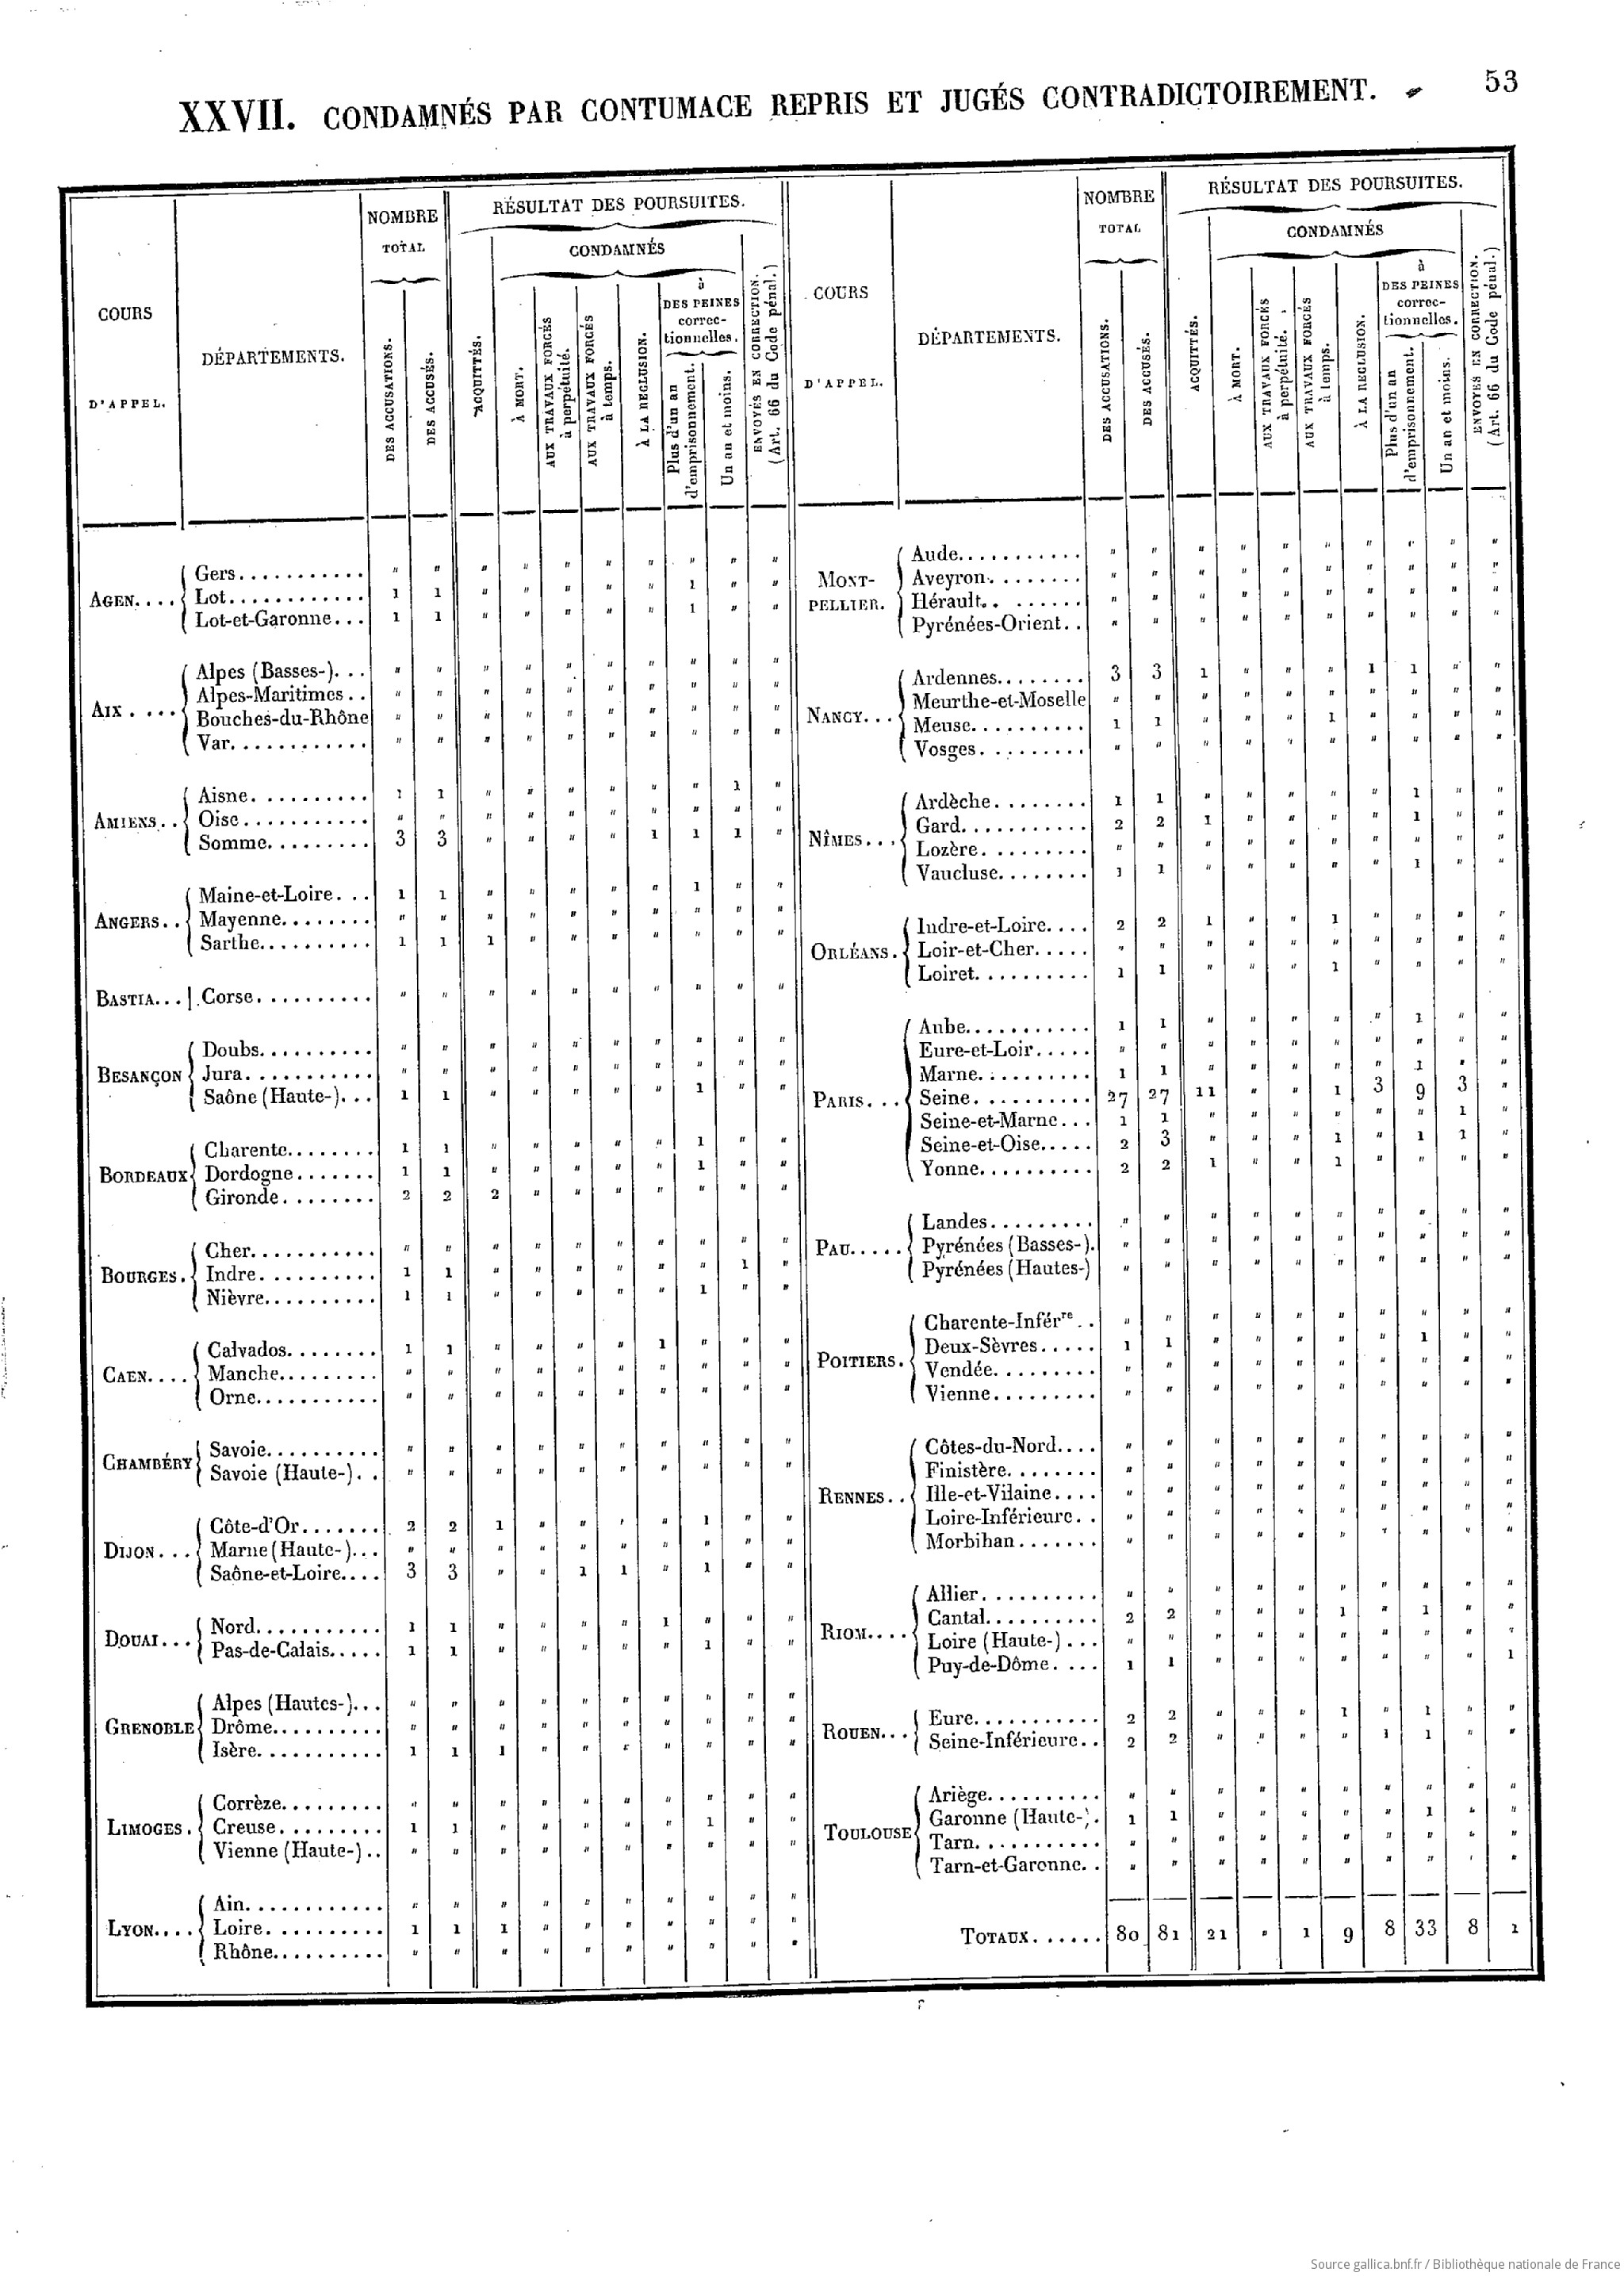
\includegraphics[width=0.7\linewidth]{Figures/Partie 3/Fig.3.3 - Compte Général.jpeg}
    \caption{Extrait du Compte Général pour 1887}
    \textit{Crédit : Gallica}
    \label{fig:Fig.3.3}
\end{figure}

\clearpage
En 1887, on compte 131 pages pour le \textit{Compte}, mais certaines années vont jusqu’à 300 pages. On voit aussi qu’il peut y avoir une difficulté sur la délimitation des zones, sujet qui a été creusé par les équipes de SocFace. 
Un projet de recherche a été mené en 2010, portant d’une part sur la saisie manuelle d’un ensemble de série extraite de ces livres, et d’autre part sur l’analyse des données ainsi obtenues\footnote{\fullcite{Sgard}}. Selon le chercheur en charge du projet, Jérôme Sgard, ces comptes ont été très peu exploités : 
\begin{quote}
    \textit{"Produit typique de l’Etat français à la fois centralisé, bureaucratique et technocratique, les Comptes de l’Administration de la Justice publiés annuellement à partir des années 1830 sont une des sources quantitatives les plus anciennes et des plus fiables disponibles sur l’histoire du pays. Or non seulement elles sont peu utilisées, en outre elles n’ont à peu près jamais été saisies de manière systématiques. Seuls quelques chapitres précis en matière criminelle, ou bien en matière de divorce ou de suicides ont fait l’objet de reconstitutions en séries temporelles de longue durée."}
\end{quote}

Il mentionne des études ponctuelles, par Emile Durkheim dans son étude sur \textit{Le suicide} en 1893 ou encore Michel Foucault pour \textit{Surveiller et Punir} en 1973. Ce genre de sources sérielles serait donc très intéressants à exploiter, particulièrement pour les informations qu’elles peuvent fournir pour les chercheurs et démographes. Ce projet a été financé par l'institut CDC pour la recherche\footnote{\href{Institut CDC pour la recherche}{https://fonda.asso.fr/institut-cdc-pour-la-recherche}}, mais les données issues du projet ne sont pas accessibles au grand public. 
Cet exemple serait une adaptation à des outils d’océrisation, mais concernant la technologie HTR, on peut penser que l’on pourrait appliquer cette technologie à d’autres corpus. La difficulté est la qualité du scripteur. Il faudrait donc un corpus appartenant à un même scripteur, avec des données d’entraînement de qualités, sur une grande variété de mots. On pourrait penser au manuscrit d’un auteur ou bien aux lettres d’un seul et même individu.\\

Le chantier d'appariement mis en œuvre par SocFace marque une nouvelle étape dans l'exploitation des données historiques, permettant une reconstitution fine des trajectoires individuelles. Au-delà de son application à la démographie historique, cette technologie ouvre des perspectives prometteuses pour d'autres corpus de données, tels que les archives judiciaires ou les manuscrits d'auteurs. En intégrant des outils d'OCR et d'HTR, SocFace non seulement enrichit la compréhension de notre passé, mais offre également un modèle adaptable pour d'autres domaines de recherche, renforçant ainsi les capacités des sciences sociales à analyser des données massives et variées.

 
	\chapter*{Conclusion}

	\addcontentsline{toc}{chapter}{Conclusion}
 Nous nous sommes donc intéressés dans ce mémoire aux acteurs qui portent ce projet, afin de réfléchir sur ce que représente pour un individu de travailler dans la recherche. Au-delà des aspects techniques, c’est la façon dont les équipes se coordonnent, dialoguent et travaillent entre elles qu’il nous a paru intéressant d’étudier. Le projet est passionnant pour les avancées technologiques qu’il réalise, et pour les résultats qu’il promet. Il va aider considérablement les équipes de recherche, spécialisées en histoire sociale de la période, mais aussi le grand public, notamment les passionnés de généalogie. Il permet de valoriser l’archive, un objet difficile à manier, qui subit son image poussiéreuse et qui est désormais plus facilement accessible. Le projet est toujours en cours, mais avance bien. Nous pourrons bientôt construire le deuxième étage de la base de données et avancer sur le chantier de l’appariement. C’est un chemin ardu mais qui aboutira à une connaissance immense des trajectoires géographiques et sociales de nos ancêtres. Tout cela est l’aboutissement d’un travail en commun efficace et précieux. Louis Henry finissait son article \textit{L’homme de l’art} sur une critique : \textit{On en parle beaucoup [de la collaboration], mais on ne cherche guère à la faciliter.} Cinquante ans plus tard, ce reproche ne tient visiblement plus. 
\newpage{\pagestyle{empty}\cleardoublepage}

%%%%%%%%%%%%%%%%%%

\appendix %Des appendices: tables figures, etc

\chapter[Fonctionnement Général - Workflow]{Workflow du fonctionnement général}
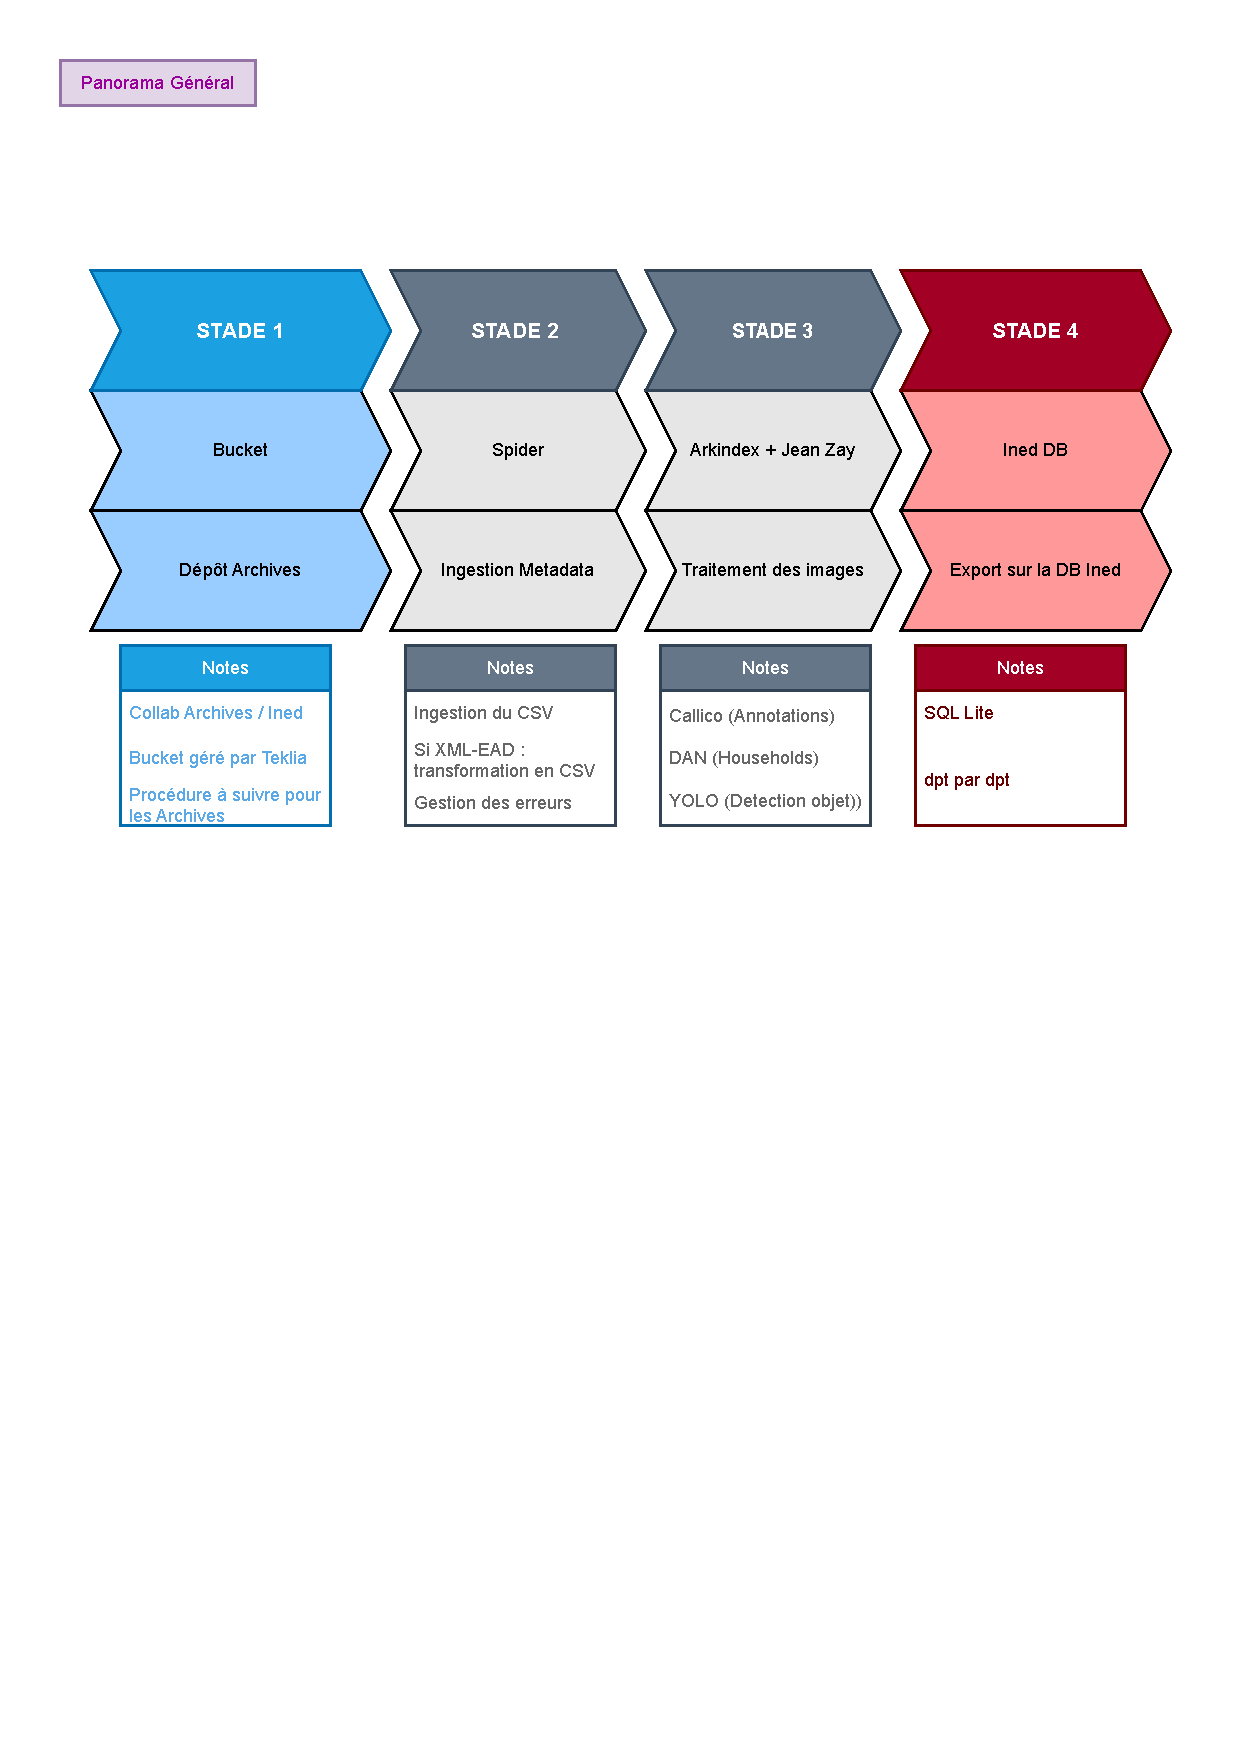
\includepdf[pages=1]{Annexe/Annexe1.pdf}

\chapter[Contacter les services d'archives - Workflow]{Contact des services d'archives}
\includepdf[pages=2]{Annexe/Annexe1.pdf}

\chapter[Fonctionnement Général d'Arkindex - Workflow]{Workflow du fonctionnement général d'Arkindex}
\includepdf[pages=3]{Annexe/Annexe1.pdf}

\chapter[Fonctionnement Général de Spider - Workflow]{Workflow du fonctionnement général de Spider}
\includepdf[pages=4]{Annexe/Annexe1.pdf}

\chapter[Machine Learning workflow]{Workflow pour le fonctionnement du Machine Learning}
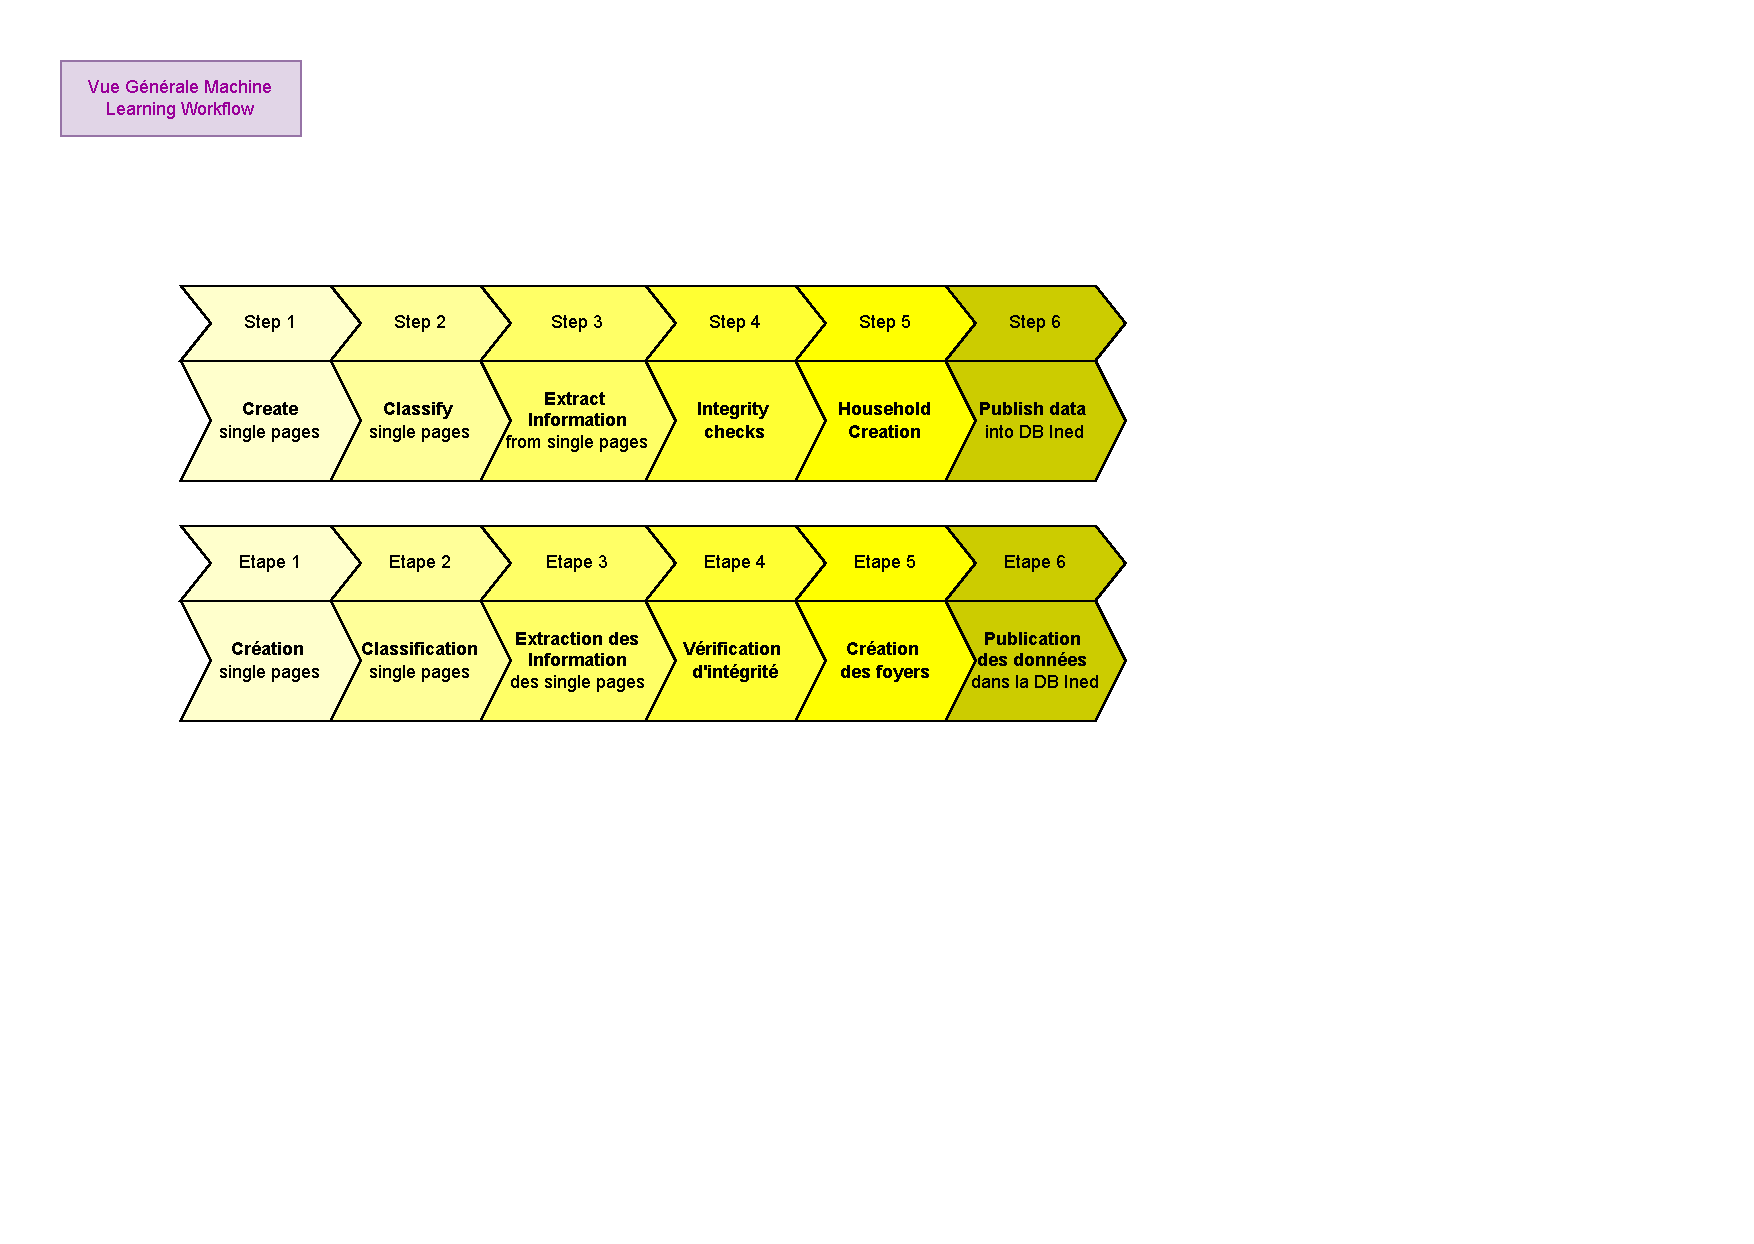
\includepdf[pages=-]{Annexe/Annexe2.pdf}

\chapter[Point mi-parcours pour les services d'archives]{Point mi-parcours pour les services d'archives}
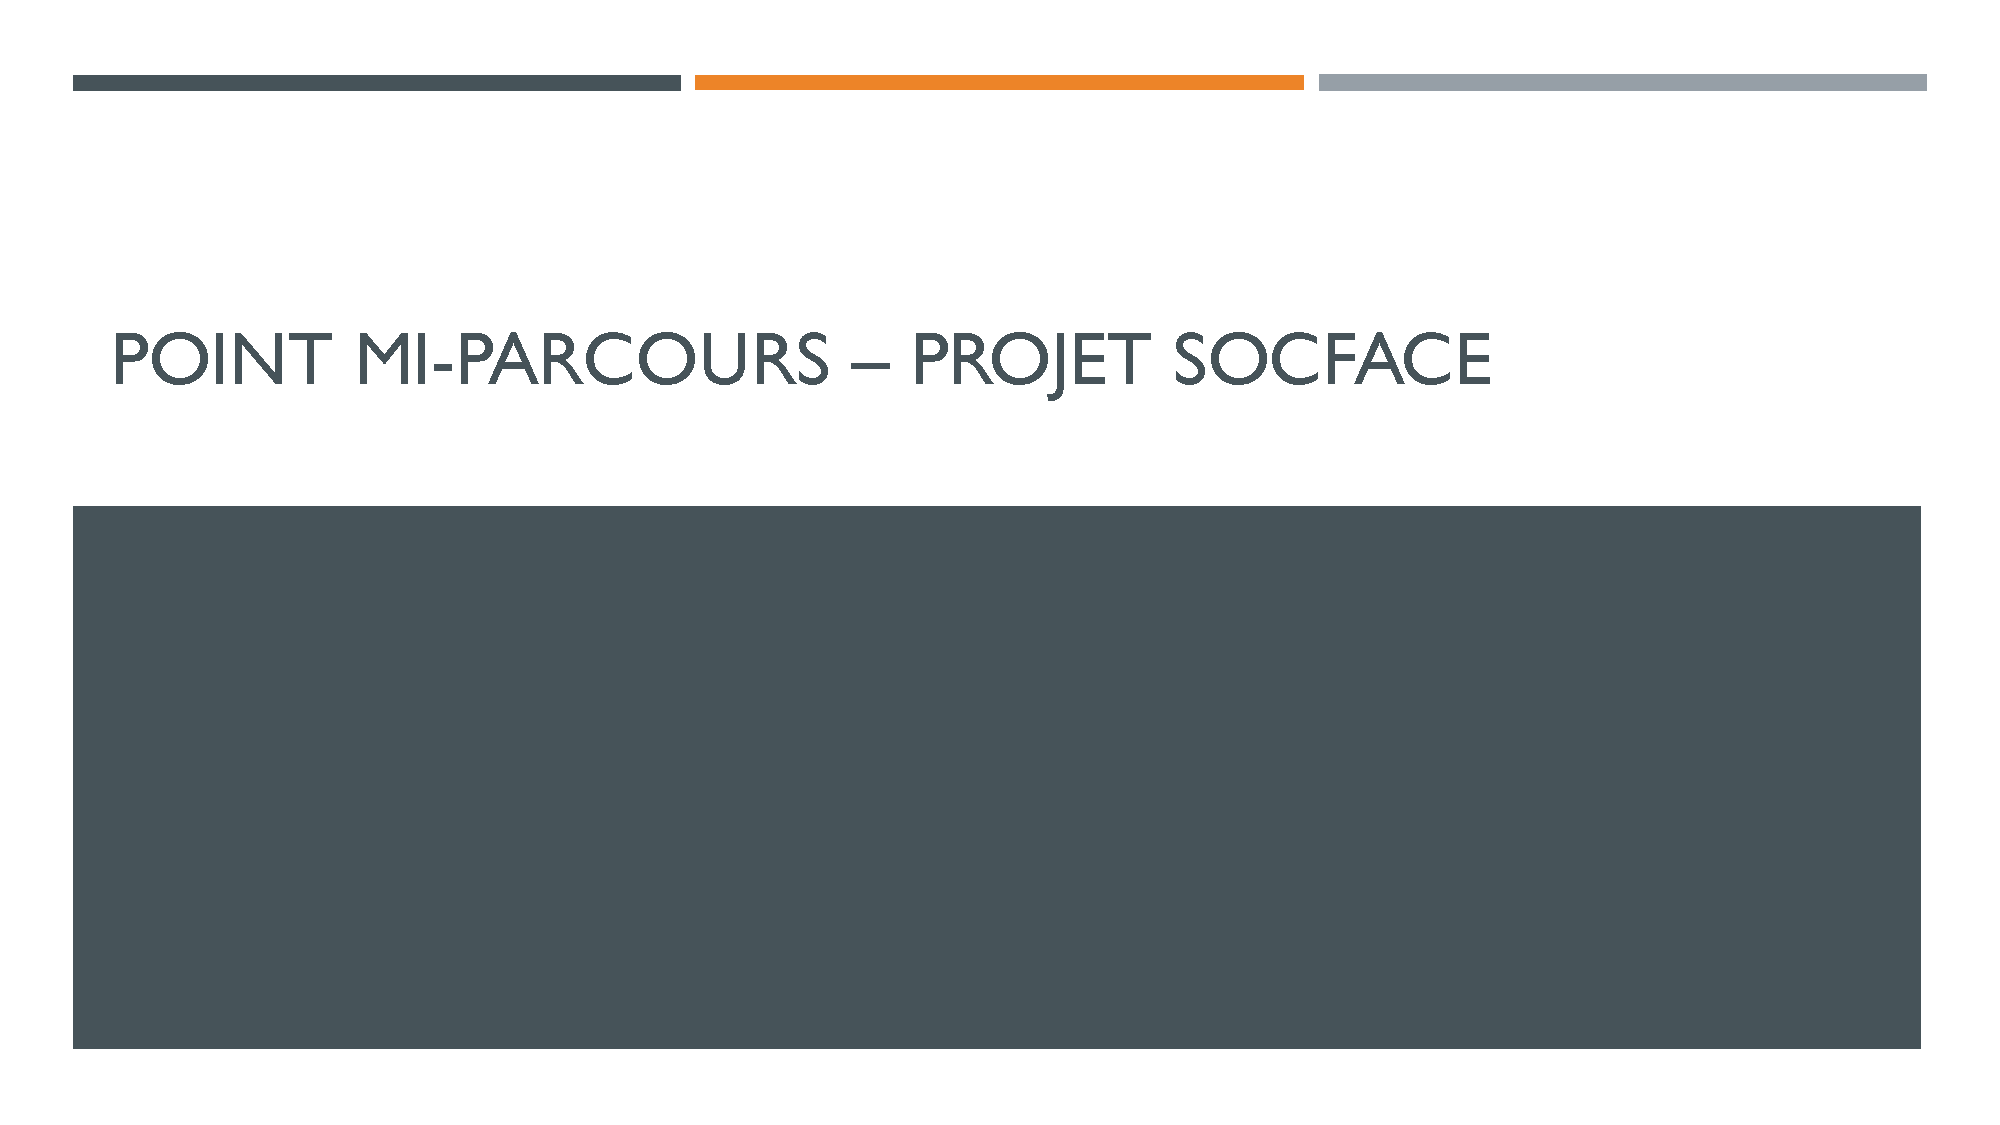
\includepdf[pages=-]{Annexe/Annexe3.pdf}\

\chapter[Consignes pour les annotateurs (Teklia)]{Consignes pour les annotateurs (Teklia)}
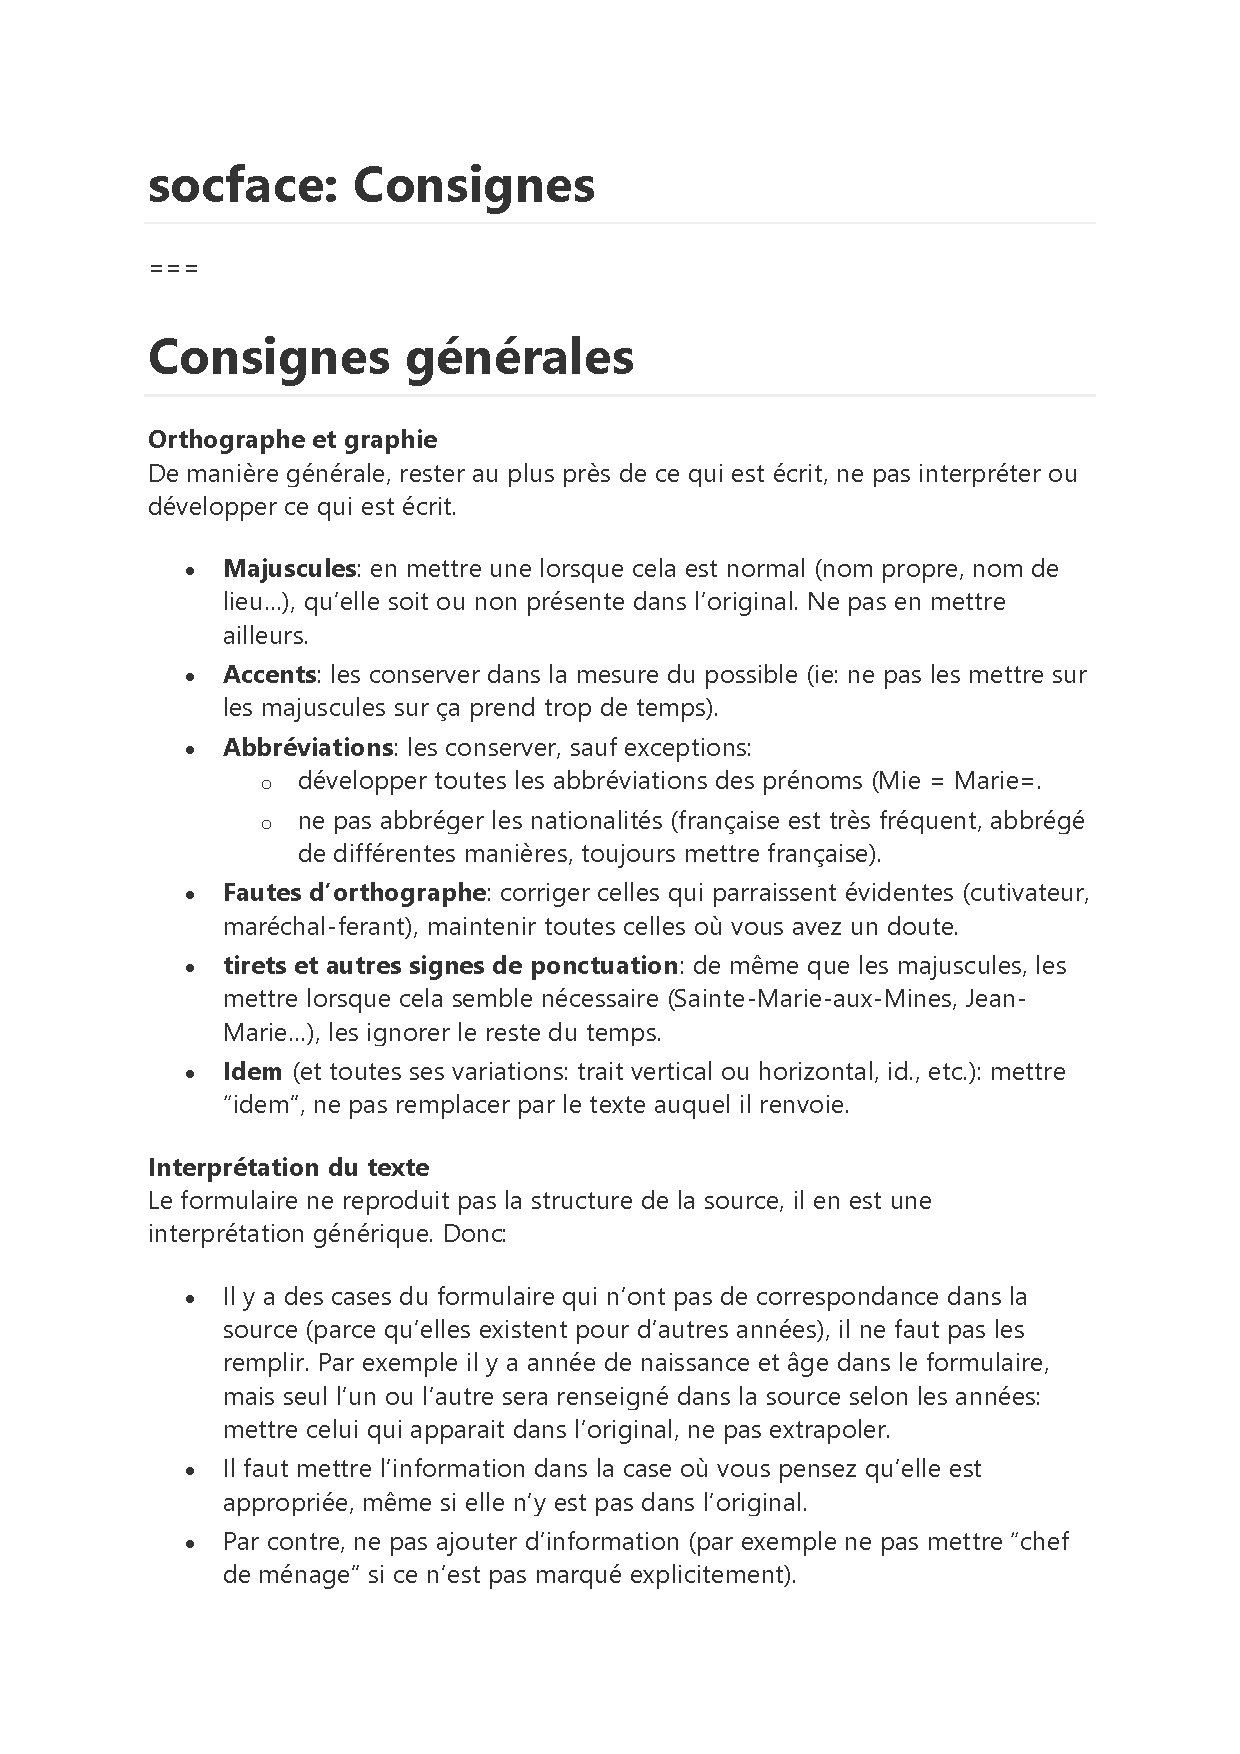
\includepdf[pages=-]{Annexe/Annexe4.pdf}


\newpage{\pagestyle{empty}\cleardoublepage}
%\pagestyle{headings} % Réinitialiser le style pour les sections suivantes

%%%%%%%%%%%%%%%%%%

\backmatter % glossaire, index, table des figures, table des matières.. (la bibliographie a déjà été appelée)

%\printindex
\printglossaries
\newpage{\pagestyle{empty}\cleardoublepage}

\listoftables
\newpage{\pagestyle{empty}\cleardoublepage}

\listoffigures
\newpage{\pagestyle{empty}\cleardoublepage}

\tableofcontents
\newpage{\pagestyle{empty}\cleardoublepage}

\end{document}
